\documentclass[a4paper,11pt]{article}

\usepackage[T1]{fontenc}
\usepackage[utf8]{inputenc}
\usepackage{graphicx}
\usepackage{longtable}
%\usepackage{xcolor}
\usepackage{hyperref}
\usepackage{indentfirst}
\usepackage{titlesec}
\usepackage[table,xcdraw]{xcolor}
\usepackage{subcaption}
\usepackage{incgraph,tikz}
\usepackage{float}
\usepackage{blindtext}
\usepackage{titlesec}
\usepackage[english]{babel}
\usepackage[utf8]{inputenc}




\setcounter{secnumdepth}{5}

\renewcommand\familydefault{\sfdefault}
\usepackage{tgheros}
%\usepackage[defaultmono]{droidmono}

\usepackage{amsmath,amssymb,amsthm,textcomp}
\usepackage{enumerate}
\usepackage{multicol}
\usepackage{tikz}
\usepackage{tabularx}
    \newcolumntype{L}{>{\raggedright\arraybackslash}X}
\usepackage{ltablex}
\usepackage{mathptmx}%

\usepackage{geometry}
\geometry{left=25mm,right=25mm,%
bindingoffset=0mm, top=20mm,bottom=20mm}


\linespread{1.3}

\newcommand{\linia}{\rule{\linewidth}{0.5pt}}

% custom theorems if needed
\newtheoremstyle{mytheor}
    {1ex}{1ex}{\normalfont}{0pt}{\scshape}{.}{1ex}
    {{\thmname{#1 }}{\thmnumber{#2}}{\thmnote{ (#3)}}}

\theoremstyle{mytheor}
\newtheorem{defi}{Definition}


% custom footers and headers
\usepackage{fancyhdr}
\pagestyle{fancy}
\lhead{}
\chead{}
\rhead{}
\lfoot{}
\cfoot{}
\rfoot{Page \thepage}
\renewcommand{\headrulewidth}{0pt}
\renewcommand{\footrulewidth}{0pt}

%no indent setting
\setlength\parindent{0pt}

% code listing settings
\usepackage{listings}
%set name to  be nothing but a number
\renewcommand\lstlistingname{ }

%
\lstset{
    language=Java,
    basicstyle=\ttfamily\small,
    %aboveskip={1.0\baselineskip},
    %belowskip={1.0\baselineskip},
    columns=fixed,
    extendedchars=true,
    breaklines=true,
    tabsize=4,
    prebreak=\raisebox{0ex}[0ex][0ex]{\ensuremath{\hookleftarrow}},
    frame=lines,
    showtabs=false,
    showspaces=false,
    showstringspaces=false,
    keywordstyle=\color[rgb]{0,0,0.255},
    commentstyle=\color[rgb]{0.133,0.545,0.133},
    stringstyle=\color[rgb]{01,0,0},
   % numbers=left,
    %numberstyle=\small,
    %stepnumber=1,
    %numbersep=10pt,
    %captionpos=t,
    %escapeinside={\%*}{*)}
}
%%%----------%%%----------%%%----------%%%----------%%%
\usepackage{pdfpages}
\usepackage{longtable}
\usepackage{graphicx}
%\usepackage{subfigure}
\usepackage{adjustbox}
\usepackage{algorithm} 
\usepackage{algpseudocode} 
\usepackage[nottoc]{tocbibind}
\begin{document}


\begin{center}

\vspace{40mm}

{\Huge \textbf{Bachelor Thesis}}\\[0.2cm]
{\large Uncertainty in Graph Neural Networks, applied within Quantum Chemistry}\\[0.2cm]

\vspace{20mm}

\begin{tabular}{cc}
\textbf{Name}: & \textbf{Student number:} \\ 

Lars Lohmann & s173875 \\
\end{tabular}

\vspace{30mm}

\begin{tabular}{cc}
\textbf{Supervisor:} & \textbf{Title:} \\
Mikkel Nørgaard Schmidt & Associate Professor\\
\end{tabular}

\vspace{20mm}

\begin{tabular}{cc}
\textbf{Department:}\\
Department of Applied Mathematics and Computer Science, Technical University of Denmark\\
\end{tabular}


\vspace{20mm}


\begin{figure}[H]
\centering

\includegraphics[width=8 cm]{Images/DTU_Logo_Hvid.jpg}
\end{figure}



\end{center} 




\pagebreak
\section{Abstract}


\newpage



\tableofcontents \newpage
\newpage
\section{Acknowledgements}
The completion of this project would not have been possible without the dedicated supervisor efforts from Mikkel Nørgaard Schmidt.\\

Mikkel Nørgaard Schmidts help has manifested through all of the stages of the project, from planning, to scoping, to executing and finalizing. His inviting presence allows for curiosity to an extend very few prior of prior supervisors have managed. His own curiosity towards the topic is contagious. His direct and fair questions and advice, has contributed to the bettering of the project, and a deepening of the knowledge around the subject matter. \\

When things get tough, his calming manner gave the mental surplus that was needed to finalize the work, and deliver on this project. \\

I would recommend his counselling efforts to any student at DTU, whether it being in a project or teaching capacity.\\

Thank you!\\

Lars Lohmann
\newpage
\section{Introduction}\label{sec:intro}

The implications of predicting molecular properties and dynamics have both large industrial- and research implications within
the natural- and life-sciences. The large amounts of compute, necessary for simulation, often makes desirable metrics intractable
to estimate. The efforts of this study, will help provide tools for industry to reduce lead time and risk in development fields
such as drug discovery and material sciences for energy storage\cite{Busk2021}.  \\

These interests, have for many years been supported by research and development methods within
the traditional field of chemistry, with emphasis on estimation techniques, that carry a heavy computational load like traditional
molecular dynamics (MD)\cite{Behler2011} or Density Functional Theory\cite{Busk2021}. Therefore, despite the emergence of
cloud-data-centers and power full algorithms available at lower cost to research, some problems still exist which are intractable
with known methods.\\

That fact, has prompted the emergence of the computational fields within Artificial Intelligence (AI), such as Machine Learning (ML),
Deep Learning (DL) and Geometric Deep Learning (GDL), to enrich the solution space. These methods produce models which tries to
decrease the lead time for predictions, while maintaining an acceptable error-rate\cite{Gasteiger2020}. Specifically the field
of Geometric Deep Learning, has emerged with a viable set of data-driven methods, for predicting molecular properties and
dynamics\cite{Atz2021}. Geometric Deep Learning comprises a set of methods, which tries to enrich the initial data structures
with a geometric prior through the structuring of data in i.e graphs, which is comprised of nodes and edges
between nodes\cite{Atz2021}. Examples of encoded information could be distances, angles or directions between nodes,
as well as symmetry properties namely equivariance or invariance.\\

Since significant risk is embodied in the task of predicting chemical and biochemical dynamics, due to end-uses often being
utilized in pharmaceutical products, proper mechanisms for estimating the the uncertainty around prediction methods, and
mitigating the impact of high uncertainty through calibration, are needed. Traditionally, data-driven methods within machine
learning and deep learning, have problems with providing the necessary uncertainties, on the metrics being predicted, making
calibration for more robust overall performance hard\cite{Song2019}\cite{Busk2021}\cite{AleatoricAndEpistemic}.
Providing methods for estimating uncertainty, and calibrating, would allow for defaulting to more traditional methods
for estimating chemical properties, when uncertainty is high in the data-driven models\cite{Busk2021}. \\

In support of producing such methods, uncertainty, can effectively be distinguished between two concepts,
namely epistemic- and aleatoric- uncertainty\cite{Busk2021}\cite{AleatoricAndEpistemic}. Aleatoric, also known as statistical
uncertainty, refers to the uncertainty inherent in experimental outcomes, due to random effects. This class of uncertainty is
classified as irreducible, due to no amount of additional information in the modelling effort, being able to reduce this type
of uncertainty\cite{AleatoricAndEpistemic}. Epistemic, also called systemic uncertainty, refers to the uncertainty in a model,
produced by lack of information, and can therefore be reduced. These two elements of uncertainty are considered by researchers
to be the sole components of total uncertainty, their sum being equal to total uncertainty in an
experiment\cite{AleatoricAndEpistemic}.\\

This paper is concerned with the task of molecular estimation of a single property, namely the binding energy in a catalyst process
between a transition metal, and a ligand\cite{Meyer2018}. The objective is to compare two ensembles of machine learning models
that try to predict the binding energy, with similar architecture, but different hyperparameters in their internal representations
of molecules, namely the state representation of scalar- and vector-properties of graphs. The main contribution of this paper,
will be to assess the influence of this hyperparameter on modelling performance and uncertainty, through the comparison of the
ensembles. This modelling performance will be measured in both a traditional metrics namely the Mean Squared Error between the
regression metric and the target, but also the uncertainty in the ensembles, produced by changing the hyperparameters to
a different value. \\

Specifically, this paper will utilize a Message Passing Neural Network (MPNN) architecture inspired by the
PAINN architecture\cite{PAINN}, to ingest graph representations of molecules, with Cartesian coordinates, atom-types and lengths
of the bonds in molecules, in order to predict the binding energy in kcal per mol. This model structure, will be provided with
a different set of internalt state complexity, and placed in two seperate uniformly weighted mixture models, one with higher sophistication
and one with lower.
The MPNN models will provide individual estimates of the target value in the test-set, where the mean and variance of the ensembles
will be the bedrock for ensemble predictions and uncertainty estimations, inspired by\cite{Lakshminarayanan2016}, and \cite{Tran2019}.\\

Specifically, this paper asks:

\begin{center}
  \textbf{\textit{Does the size of internal state representations, impact prediction error and uncertainty in ensembles of
      Message Passing Neural Networks}}
\end{center}

The following sections of this paper, namely[\ref{sec:intro},\ref{sec:definitions},\ref{sec:theory}],
we will go through relevant concepts and theories, necessary for assessing the results and methods in this paper.
This is followed by a description of the experimental methods, and a presentation of the data set,
on which the methods have been utilized in sections[\ref{sec:methods},\ref{sec:data}].
Lastly, results followed by a conclusion and a discussion of the potential points of error,
which influence the outcomes of the experiment in sections[\ref{sec:results},\ref{sec:discussion},\ref{sec:conclusion}].

\newpage



\section{Theory}\label{sec:theory}

In this section, we will discuss the theoretical foundations of message passing neural networks (MPNNs) and ensembles for predicting
the binding energy of molecules in a catalyst process. The section will start with a note on symmetry, specifically detailing the
usage of invariant and equivariant representations in the model. Moving on to a detailing of the modelling architecture, ending in a
presentation of the ensemble structure and metrics used in the experiment.

\subsection{Symmetry}\label{sec:symmetry}
A large part of the contribution from the PAINN paper\cite{PAINN}. is the emphasis on building and modelling equivariant features.
The interest in equivariance, comes from the ability to express more information about a graph structure, at a lower level of
computational cost. This ties in with the search for modelling approaches that descrease lead-time on predictions, while maintaining an
acceptable error-rate.
let $\vec{\mathbf{x}}$ be a feature, and $o$ denote an operation.
$\vec{\mathbf{x}}$ is a rotational equivariant feature, under the operation $o$,
if the below equation is satisfied for any rotation matrix $R \in \mathbb{R}^{3 \times 3}$\ref{eq:equivariant}:

\begin{equation}\label{eq:equivariant}
    R \vec{\mathbf{o}}(\vec{\mathbf{x}}) = \vec{\mathbf{o}}(R \vec{\mathbf{x}})
\end{equation}

And $\vec{\mathbf{x}}$ is a rotational invariant feature, under the operation $o$,
if the below equation is satisfied for any rotation matrix $R \in \mathbb{R}^{3 \times 3}$\ref{eq:invariant}:

\begin{equation}\label{eq:invariant}
    \mathbf{o}(\vec{\mathbf{x}}) = \mathbf{o}(R \vec{\mathbf{x}})
\end{equation}

In order to detail whether any of these equations hold, one needs to consider which operations, make this the statements true for
directional information. The paper of inspiration \cite{PAINN} highlights a list of operations,
that equivariant MPNN's in particular can use in order to preserve equivariant information properties on their features:

\begin{itemize}
    \item Any (nonlinear) function of scalars: $\mathbf{f}(\mathbf{s})$
    \item Scaling of vectors $ \mathbf{s} \circ \vec{\mathbf{v}}$
    \item Linear combinations of equivariant vectors: $\mathbf{W} \vec{\mathbf{v}}$
    \item Scalar products: $\mathbf{s} = \left \| \vec{\mathbf{v}} \right \|^{2}, s = \left \langle \vec{\mathbf{v}}_{1}, \vec{\mathbf{v}}_{2} \right \rangle$
    \item Vector products: $\vec{\mathbf{v}}_{1} \times \vec{\mathbf{v}}_{2}$
\end{itemize}

This list entails a linearity constraint on the operations on equivariant features\cite{PAINN}. If the linearity constraint is
not satisfied, then the feature will not be equivariant, and directional information will not be preserved.

The subsequent section presents
a number of features (presented also as representations below) and operations relevant to the MPNN.
These need not all be equivariant, invariant, linear or non-linear. What constitutes an equivariant MPNN in the eyes of
Schütt et. al.\ref{PAINN}, is not that all operations on directional information are linear, and equivariance is preserved globally.
As long as an equivariant representation containing directional information, is obeying  the constraints of the list above and thereby
equation\ref{eq:equivariant}, directional information is preserved, and can be allowed to diffuse through the model representations.

\subsection{Message Passing Neural Networks}\label{subsec:modelling_task}

The key idea behind MPNNs is the concept of
message passing, where each node in the graph exchanges information with its neighbors in an iterative manner.

Let $G = (N, E)$ be a graph, where $N$ is the set of nodes and $E$ is the set of edges.
Each node $n \in N$ is associated with an invariant representation vector $\mathbf{S}_{n} \in \mathbb{R}^{Fx1}$,
an equivariant representation
vector $\vec{\mathbf{v}}_{n} \in \mathbb{R}^{Fx3}$ and a position in 3D space $\vec{r}_{i} \in \mathbb{R}^3$.
$F$ denotes the number of features in the state representation (in our case, $F = 64$ and $F = 128$).
Each edge $(i, j) \in E$ is associated with vector difference $\vec{r}_{ij} = \vec{r}_{i} - \vec{r}_{j}$.
A node $n_{j} \in N$ is said to be a neighbour of a node $n_{i} \in N \setminus \{n_{j}\} = \mathcal{N}(i) $
if $n_{j}$ is within the cutoff distance of $n_{i}$: $\mathcal{N}(i) = \{j |\lVert \vec{r}_{ij} \rVert \leq r_{cut}  \}$.


The message passing process in an MPNN can be described by the following equations \ref{eq:message_block} and \ref{eq:update_block}
following the notation of \cite{PAINN}.

\begin{equation}\label{eq:message_block}
    \vec{\mathbf{m}}_{i}^{v,t+1} = \sum_{j \in \mathcal{N}(i)} \vec{M_t}(\mathbf{S}_{i}^{t}, \mathbf{S}_{j}^{t}, \vec{\mathbf{v}}_{i}^{t}, \vec{\mathbf{v}}_{j}^{t}, \vec{r}_{ij})
\end{equation}

\begin{equation}\label{eq:update_block}
    \vec{\mathbf{s}}_{i}^{v,t+1} = \vec{U_t}(\mathbf{S}_{i}^{t}, \vec{\mathbf{v}}_{i}^{t}, \vec{\mathbf{m}}_{i}^{v,t+1})
\end{equation}

The $U$ and $M$ functions respectively being the update, and message functions, taking into account scalar, vector and
directional features. These equations utilize both invariant and equivariant representations, letting
representations interact, in accordance with knowledge surrounding the chemical descriptor trying to be predicted. The underlying
operations of the functions $U$ and $M$, have a linearity constraint on equivariant representations of directional information,
in order to maintain
information, throughout the modelling process\cite{Atz2021}. The message and update functions will be designed, such that scalars $\mathbf{s}_{i}$
and vectors $\vec{\mathbf{v}}_{i}^{t}$ are updated in an iterative manner via the output residuals $(\Delta \mathbf{s}_{i}^{t}, \Delta \vec{\mathbf{v}}_{i}^{t})$ produced by the message and update functions.
this entails that for the message block output is:

\begin{equation}\label{eq:residual_message}
    \sum_{j \in \mathcal{N}(i)} \vec{M_t}(\mathbf{S}_{i}^{t}, \mathbf{S}_{j}^{t}, \vec{\mathbf{v}}_{i}^{t}, \vec{\mathbf{v}}_{j}^{t}, \vec{r}_{ij}) = (\Delta \mathbf{s}_{i}^{m}, \Delta \vec{\mathbf{v}}_{i}^{m})
\end{equation}

And for the update block output is:

\begin{equation}\label{eq:residual_update}
    \vec{U_t}(\mathbf{S}_{i}^{t}, \vec{\mathbf{v}}_{i}^{t}, \vec{\mathbf{m}}_{i}^{v,t+1}) = (\Delta \mathbf{s}_{i}^{u}, \Delta \vec{\mathbf{v}}_{i}^{u})
\end{equation}

These residuals will be further developed in the sections coming.


\subsubsection{Message Block}\label{subsubsec:message_block}

Further, we define the residual update of invariant scalar\ref{eq:residual_scalar}-representations in the message block,
based on the expression derived earlier in equation\ref{eq:residual_message}:

\begin{equation}\label{eq:residual_scalar}
    \Delta \mathbf{s}_{i}^{m}= (\phi_{s}(\mathbf{s}) * \mathcal{W}_{s})_{i} = \sum_{j} \phi_{s}(\mathbf{s}) \circ \mathcal{W}_{s} \left ( \left \| r_{ij} \right \| \right )
\end{equation}

Worht mentioning about the above expression, are that the index 's' refers to a certain split of the $\phi \circ W$-product seen
in figure\ref{img:message_block}. All indexes of 's', 'v', or a combination of the two in the below equations,
will be detailing what part of a split it belongs to. This comes down to $\phi$ and $\mathcal{W}$ being shared networks, that are re-used
for multiple parts of the modelling.
Following the above equation\ref{eq:residual_scalar}, two expression are utilized, namely $\phi_{s}$ and $\mathcal{W}_{s}$.
$\phi_{s}$ represents atomwwise layers, which have undergone transformations through two linear layers and a SiLU-function,
introducing some non-linearity potentially for better gradient flow, via the smooth gradient. Conceptually it can be interpreted as an
expansion of the embedded atomwise neighbours of a node.
Let $f(x)$ denote a linear layer:

\begin{equation}\label{eq:linear_layer}
    f(x) = w \cdot x + b
\end{equation}

and $SiLU(x)$ denote the SiLU-function:

\begin{equation}\label{eq:SiLU}
    SiLU(x) = x \cdot \left (  \frac{1}{(1+e^{-x}))}\right )
\end{equation}

Then $\phi$ is defined as:

\begin{equation}\label{eq:phi}
    \phi_{s}(\mathbf{s}) = f_{1}(SiLU(f_{2}(\mathbf{s})))
\end{equation}

Worth noting about the above equation\ref{eq:phi}, are the indexes of the linear layers. These are maintained to emphasize,
the individuality of their parameters throughout the whole modelling process.

The rotationally invariant filters $\mathcal{W}_{s}$ are defined as, are linear combinations of a radial basis function
(RBF)\ref{eq:rbf}\cite{Atz2021}. The radial basis function outputs are chosen such that it is centered around twenty
points, $ C = \{1, 2, 3, \ldots, 20\}$. These twenty points are centers of the filter, and their units are Angstrom.
These centers are chosen, such that they cover all distances in the data set, which is confirmed in a later section\ref{distances}.
The expansions provide a representation of similarity or dissimilarity, between the input relative position $\vec{r}_{ij}$,
and the chosen points $C$ \cite{rbf}.
The function takes directional information $\lVert \vec{r}_{ij} \rVert$ and a cutoff
$r_{cut}$. The rbf acts as filter generating function\cite{Schütt2017},
effectively quantizing the directional information. The function is defined as:

\begin{equation}\label{eq:rbf}
    \mathbf{RBF}(\lVert \vec{r}_{ij} \rVert) = \sin \left( \frac{C \pi}{r_{cut}} \cdot \lVert \vec{r}_{ij} \rVert  \right) / \lVert \vec{r}_{ij} \rVert
\end{equation}

This radial basis is then expanded on by a linear layer $f$, before the cosine cutoff function is applied. This effectively means that,
that atoms beyond the cutoff radius, does not contribute to the representation\cite{Behler2011}. The cosine cutoff function
is defined as:

\begin{equation}\label{eq:coscutoffproject}
    \begin{aligned}
        \mathbf{f}_{cut}(\lVert \vec{r}_{ij} \rVert) & =
        \begin{cases}
            0.5 \cdot \cos \left( \frac{\pi \lVert \vec{r}_{ij} \rVert}{r_{cut}} + 1  \right) \cdot f(\mathbf{RBF}(\lVert \vec{r}_{ij} \rVert)) & \text{if } d \leq r_{cut} \\
            0                                                                                                                                   & \text{if } d > r_{cut}    \\
        \end{cases}
    \end{aligned}
\end{equation}

Worth mentioning is that the cosine cutoff implemented in this project, has an added factor compared to Behler2011\cite{Behler2011}, namely
$f(\mathbf{RBF}(\lVert \vec{r}_{ij} \rVert))$. This is deemed missing by the project, and is therefore added. The full representation of
the rotationally invariant filters are therefore:

\begin{equation}
    \mathcal{W}_{s} = \mathbf{f}_{cut}(\lVert \vec{r}_{ij} \rVert, f_{3}(\mathbf{RBF}(\lVert \vec{r}_{ij} \rVert)))
\end{equation}

Next also utilizing continous-filter convolutions $\mathcal{W}$, we define the residual equivariant vector update,
following the definition in \ref{eq:residual_message}, from the message block as:

\begin{equation}\label{eq:residual_vector}
    \Delta \vec{\mathbf{v}}_{i}^{m}= \sum_{j} \vec{\mathbf{v}}_{j} \circ \phi_{vv}(\mathbf{s}_{j}) \circ \mathcal{W}_{vv} \left ( \left \| \vec{\mathbf{r}}_{ij} \right \| \right ) + \sum_{j} \phi_{vs}(\mathbf{s}_{j}) \circ \mathcal{W}'_{vs} \left ( \left \| \vec{\mathbf{r}}_{ij} \right \| \right ) \frac{\vec{\mathbf{r}}_{ij}}{\left \|\vec{\mathbf{r}}_{ij} \right \|}
\end{equation}

The equation\ref{eq:residual_vector} consists of two terms. The first being a convolution of an invariant filter $\phi_{vv}(\mathbf{s}_{j})$
being scaled/weighted with equivariant features $\sum_{j} \vec{\mathbf{v}}_{j} \circ \phi_{vv}(\mathbf{s}_{j})$\cite{PAINN} as well as
the rotationally invariant filters $\mathcal{text{W}}_{vv}(\lVert \vec{r}_{ij} \rVert)$. This term propagates prior directional information,
from neighbour nodes $n_{j}$ to the node $n_{i}$, stored in the equivariant representation vectors $\vec{\mathbf{v}}_{j}$,
after the initial message passing round since there is no
directional information in the initialization of the vector.
The second term is a convolution of invariant features $\phi_{vs}(\mathbf{s}_{j})$
with an equivariant filter ${W}'_{vs} \left ( \left \| \vec{\mathbf{r}}_{ij} \right \| \right ) \frac{\vec{\mathbf{r}}_{ij}}{\left \|\vec{\mathbf{r}}_{ij} \right \|}$
Which is the gradient of the invariant filter:

\begin{equation}
    \triangledown \mathcal{W}_{vs}(\lVert \vec{r}_{ij} \rVert) =  \mathcal{W}_{vs}'(\lVert \vec{r}_{ij} \rVert) \frac{\vec{\mathbf{r}}_{ij}}{\left \|\vec{\mathbf{r}}_{ij} \right \|}
\end{equation}

The gradient part of the expression $\mathcal{W}_{vs}'(\lVert \vec{r}_{ij} \rVert)$, also being an invariant filter, is modeled directly,
without taking the derivative\cite{PAINN}. This concludes the equations related to the message block. A full architectural overview
of the block, can be seen in the figure below\ref{img:message_block}:

\begin{figure}[H]
    \caption{Message Block}
    \centering\label{img:message_block}
    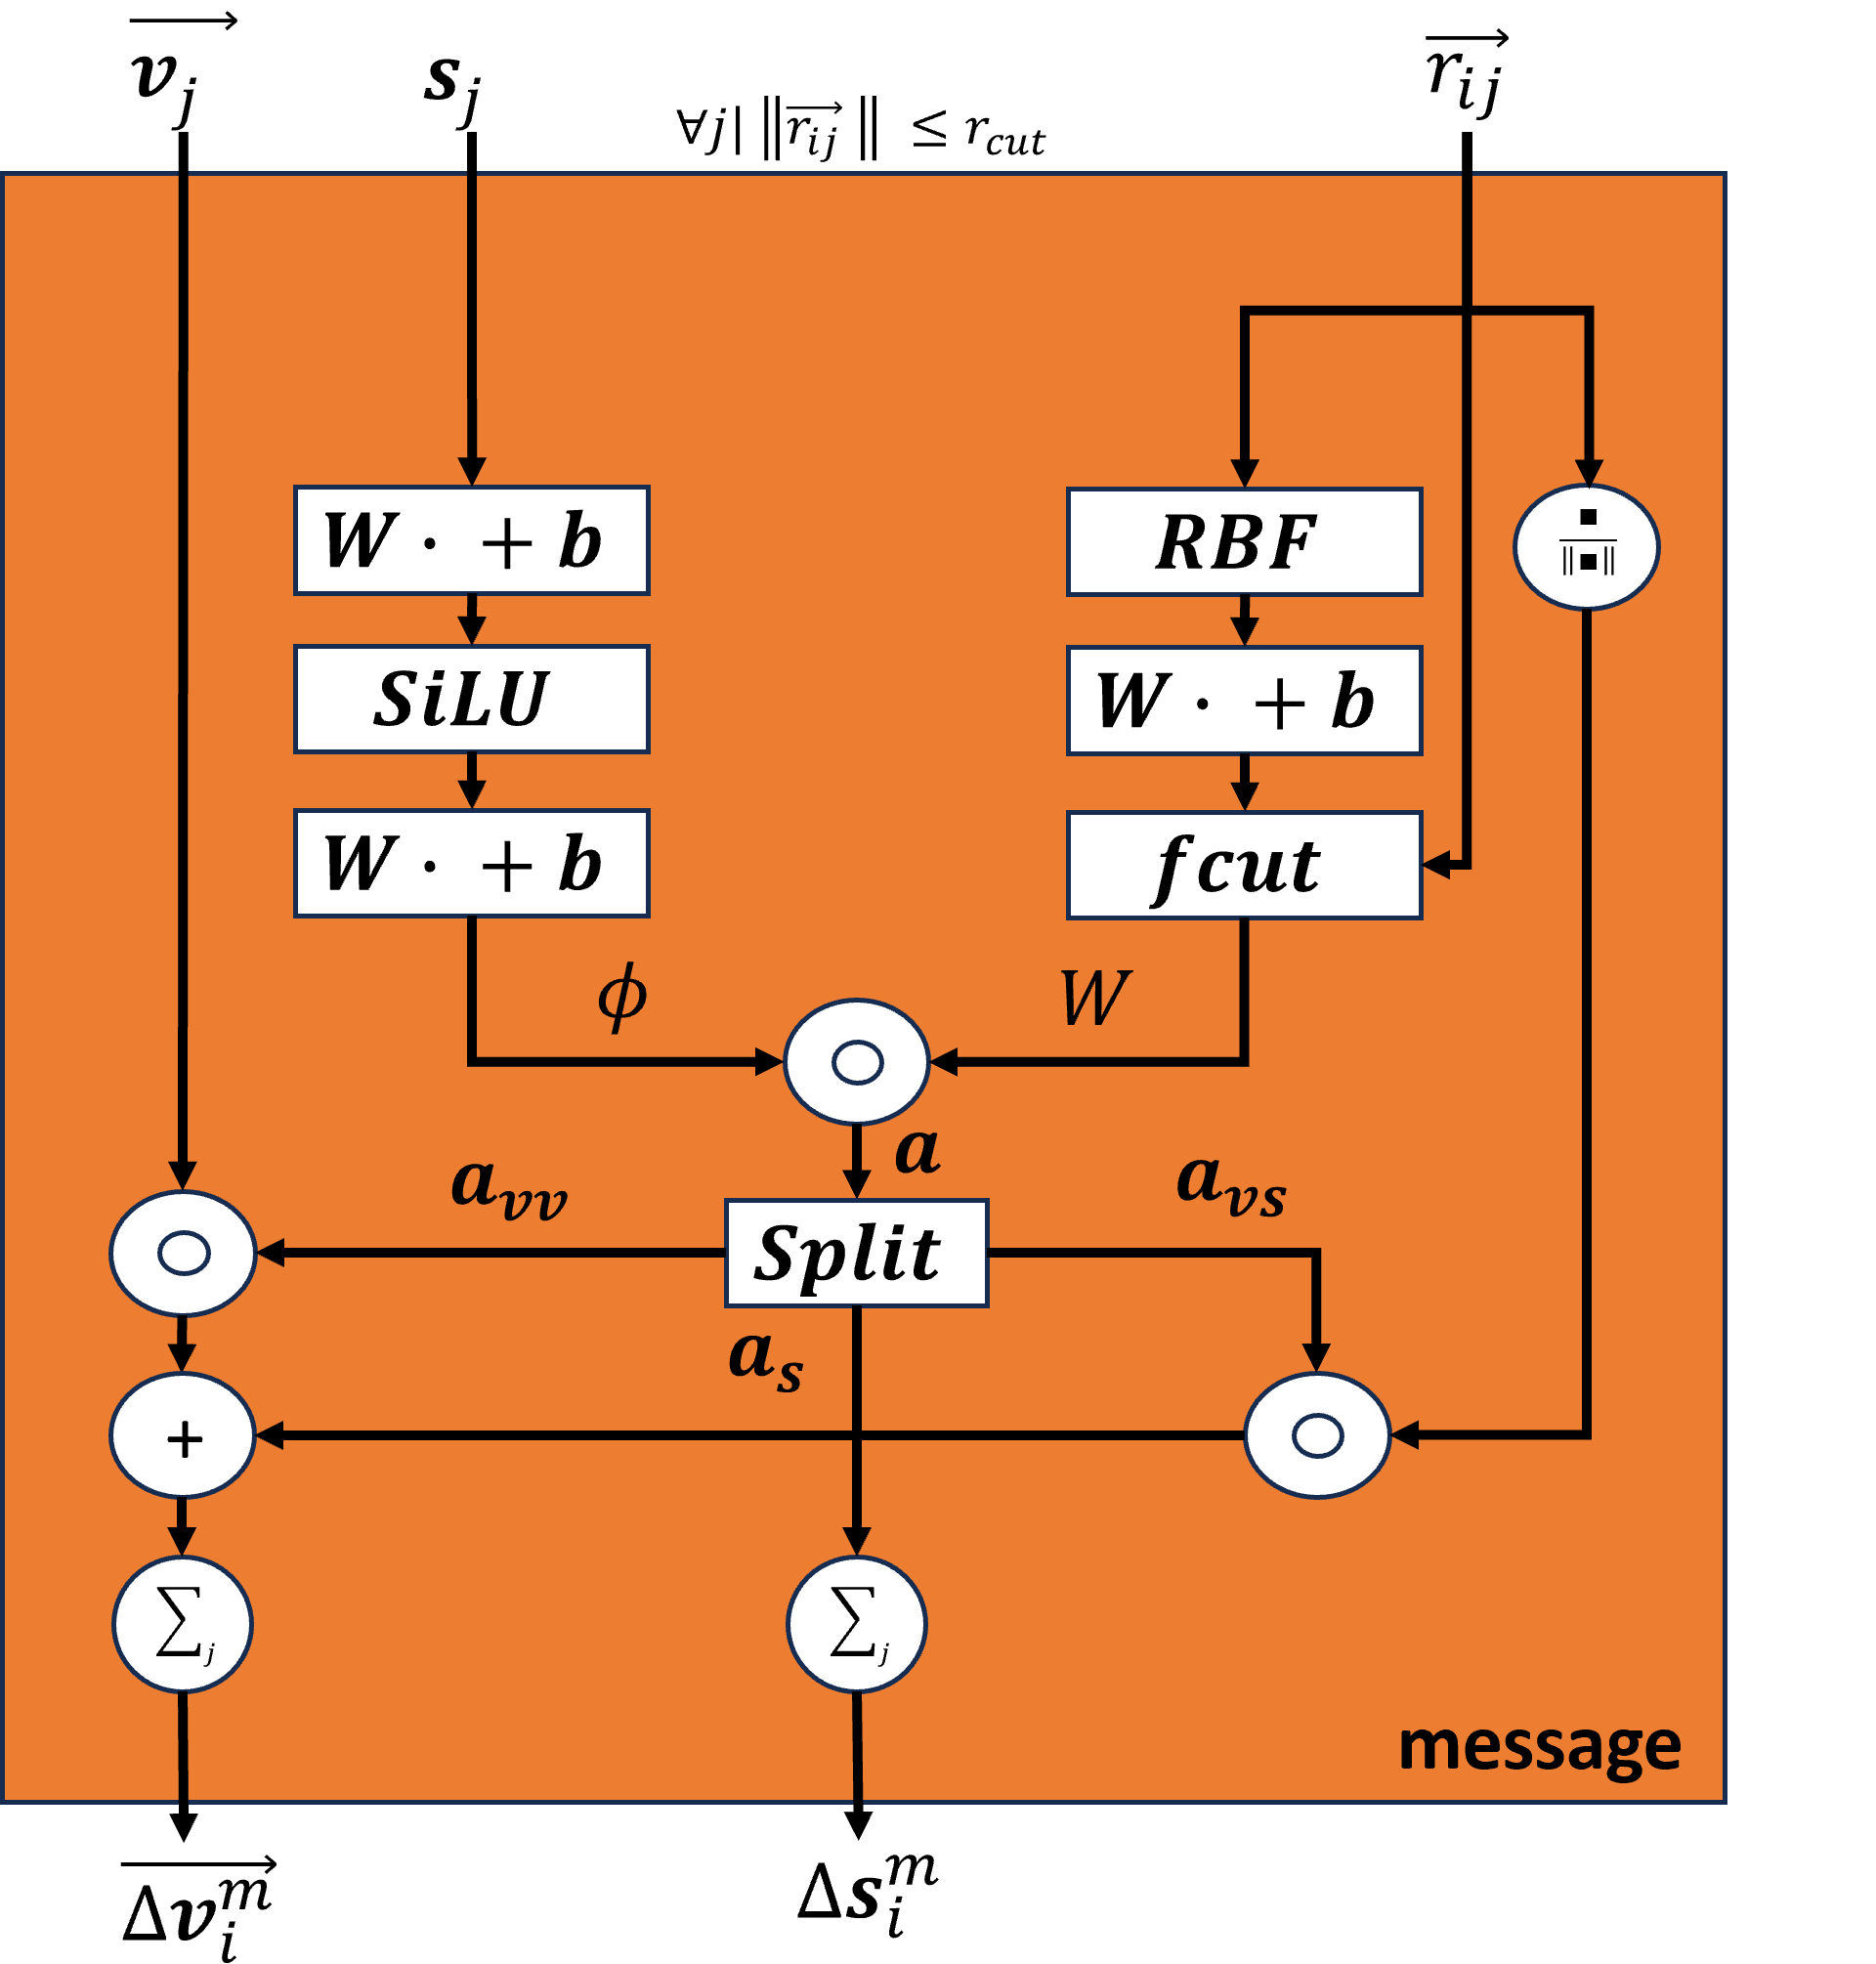
\includegraphics[width=250pt]{Images/Method/message_block.png}
\end{figure}

\subsubsection{Update Block}\label{subsubsec:update_block}

The update block builds on the information gained from the message block. It takes each individual node $n_{i} = (\mathbf{s}_{i}, \vec{\mathbf{v}}_{i})$
And runs ite through a set of transformations, before arriving at yet another set of residual update of the scalar and vector
representations respectively.

From the definition of an update function made in equation\ref{eq:residual_update}, the residual update of the invariant scalar properties
are defined for the update block as\ref{eq:residual_scalar_update}:

\begin{equation}\label{eq:residual_scalar_update}
    \Delta \mathbf{s}_{i}^{u}= \mathbf{a}_{ss} \left ( \mathbf{s}_{i}, \left \| \mathbf{V}\vec{\mathbf{v}}_{i} \right \| \right ) + \mathbf{a}_{sv} \left ( \mathbf{s}_{i}, \left \| \mathbf{V}\vec{\mathbf{v}}_{i} \right \| \right ) \left \langle \mathbf{U} \vec{\mathbf{v}}_{i}, \mathbf{V} \vec{\mathbf{v}}_{i} \right \rangle
\end{equation}

In general the update function, utilizes a shared network $a$, just as the message function did with $\phi$ and $\mathcal{W}$.
This network is defined as by inputs of the invariant scalar representation $\mathbf{s}_{i}$ and the normalized linear combination of
the equivariant vector representation $\left \| \mathbf{V}\vec{\mathbf{v}}_{i} \right \|$. both $U$ and $V$ are learned structures
by the network, and are applied inorder to produce the linear combinations of equivariant vector representations with dimensions:
$V \in \mathbb{R}^{F \times F}$ and $U \in \mathbb{R}^{F \times F}$.
The network applies two linear transformations
to the input $f$, as well a SiLU transformation $SiLU$. The full expression of $a$ can be seen in the following equation:
\begin{equation}\label{eq:a}
    \mathbf{a}(\mathbf{s}_{i}, \left \| \mathbf{V}\vec{\mathbf{v}}_{i} \right \|) = f_{4}(SiLU(f_{5}(\mathbf{s}_{i}, \left \| \mathbf{V}\vec{\mathbf{v}}_{i} \right \|)))
\end{equation}

The residual update of the scalar representations in the update block\ref{eq:residual_scalar_update} contains two terms.
The first term in\ref{eq:residual_scalar_update} relates to a non-linear scalar representation $\mathbf{a}_{ss} \left ( \mathbf{s}_{i}, \left \| \mathbf{V}\vec{\mathbf{v}}_{i} \right \| \right )$.
The second applies the scalar product of the two matrices $U$ and $V$, as further scaling to the non-linear of the invariant features $\mathbf{s_{i}}$,
as well as the coupling of the scalar representations with the normalized linear combination of the equivariant vector representation similar to the first
term. This whole expression imposes some further non-linearity on the scalar representations, as well as letting the equivariant representation
influence the output, via the scalar product, and the normalized linear combination.

The residual update of the vector representations in the update block is defined as\ref{eq:residual_vector_update}:

\begin{equation}\label{eq:residual_vector_update}
    \Delta \mathbf{v}_{i}^{u}= \mathbf{a}_{vv} \left ( \mathbf{s}_{i}, \left \| \mathbf{V}\vec{\mathbf{v}}_{i} \right \| \right ) \mathbf{U}\vec{\mathbf{v}}_{i}
\end{equation}

Which is similarly non-linear scaling $\mathbf{a}_{vv} \left ( \mathbf{s}_{i}, \left \| \mathbf{V}\vec{\mathbf{v}}_{i} \right \| \right )$
of the linear combinations of the equivariant representations, although the combinations are not normalized.

This concludes the section on the update block, a figure of the update-blocks architecture, can be found below\ref{img:update_block}.

\begin{figure}[H]
    \caption{Update block}
    \centering\label{img:update_block}
    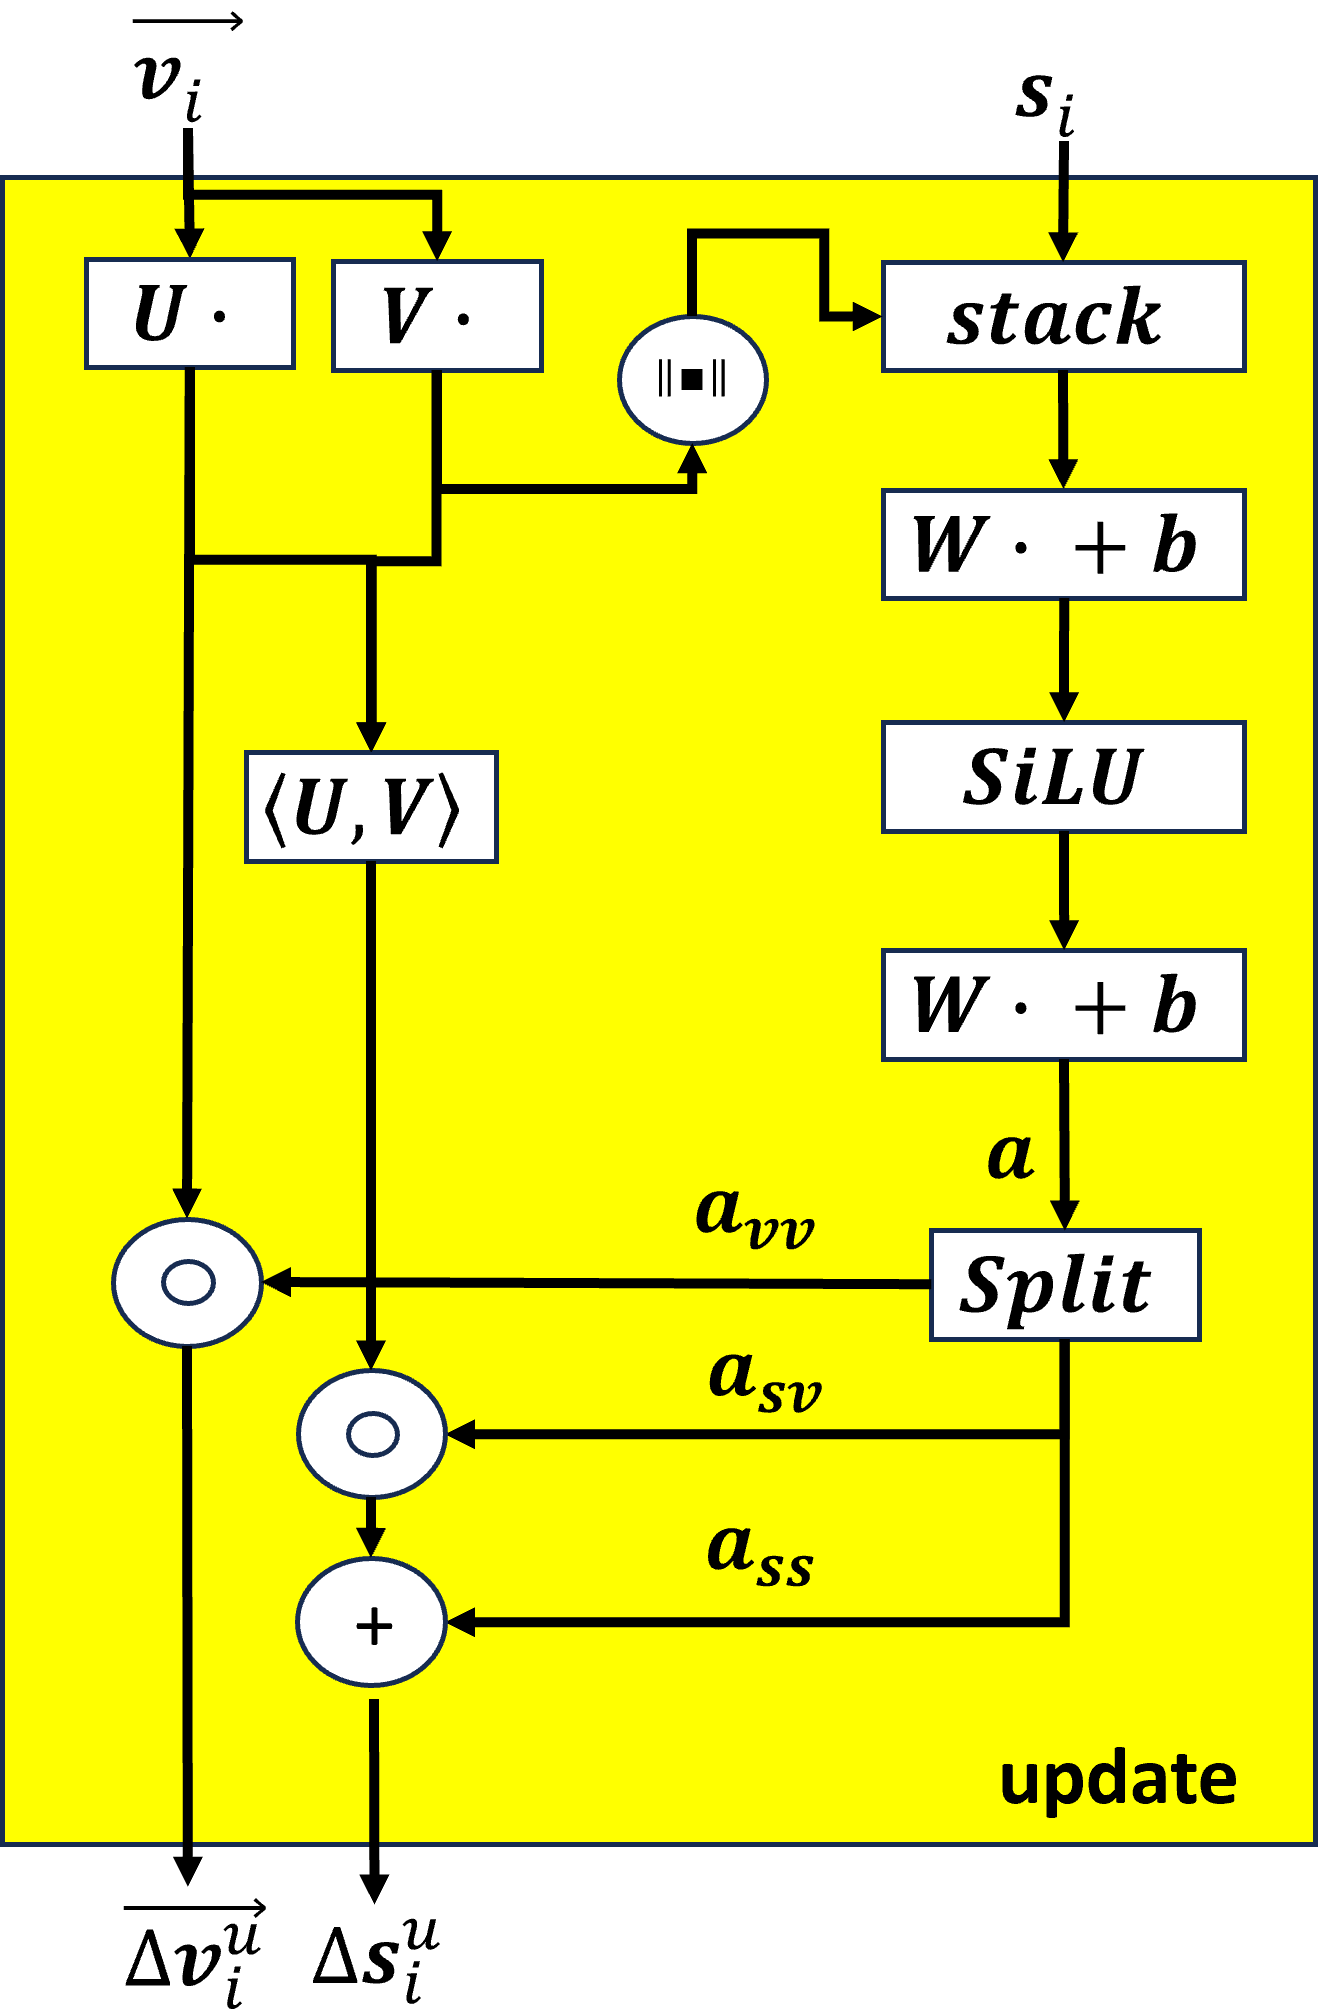
\includegraphics[width=200pt]{Images/Method/update_block.png}
\end{figure}

\subsubsection{A note on Equivariance}\label{note-equivariance}

As the initial symmetry section detailed\ref{sec:symmetry}, there are a number of operations which are valid for equivariant representations
of directional information. This section will take a short look back on the structures detailed above in the
message-\ref{subsubsec:message_block} and update-block\ref{subsubsec:update_block} sections, how exactly directional information
propagates in the network.

Directional information is propagated from vector differences $\vec{\mathbf{r}}_{ij}$ as input, into many of the model areas. The main storage
unit of directional information, is the equivariant vector representation $\vec{\mathbf{v}}_{i}$. This representation allows for directional
information to be stored across iterations, and it is therefore important that its equivariance characteristics are preserved.

If we take a look at the full set of operations applied to the vector representation, we can check for whether equivariance is preserved,
by checking the list presented in the section\ref{sec:symmetry}. The operations applied to the vector representation are as follows:

\begin{equation}\label{eq:vector_operations}
    \Delta \vec{\mathbf{v}}_{i} = \Delta \vec{\mathbf{v}}_{i}^{m} + \Delta \vec{\mathbf{v}}_{i}^{u} =
    \sum_{j} \vec{\mathbf{v}}_{j} \circ \phi_{vv}(\mathbf{s}_{j}) \circ \mathcal{W}_{vv} \left ( \left \| \vec{\mathbf{r}}_{ij} \right \| \right ) + \sum_{j} \phi_{vs}(\mathbf{s}_{j}) \circ \mathcal{W}'_{vs} \left ( \left \| \vec{\mathbf{r}}_{ij} \right \| \right ) \frac{\vec{\mathbf{r}}_{ij}}{\left \|\vec{\mathbf{r}}_{ij} \right \|} +
    \mathbf{a}_{vv} \left ( \mathbf{s}_{i}, \left \| \mathbf{V}\vec{\mathbf{v}}_{i} \right \| \right ) \mathbf{U}\vec{\mathbf{v}}_{i}
\end{equation}

we further break the expression down, into its seperate terms, we can analyse them one at a time:

\begin{equation}\label{eq:term-one}
    \sum_{j} \vec{\mathbf{v}}_{j} \circ \phi_{vv}(\mathbf{s}_{j}) \circ \mathcal{W}_{vv} \left ( \left \| \vec{\mathbf{r}}_{ij} \right \| \right )
\end{equation}

\begin{equation}\label{eq:term-two}
    \sum_{j} \phi_{vs}(\mathbf{s}_{j}) \circ \mathcal{W}'_{vs} \left ( \left \| \vec{\mathbf{r}}_{ij} \right \| \right ) \frac{\vec{\mathbf{r}}_{ij}}{\left \|\vec{\mathbf{r}}_{ij} \right \|}
\end{equation}

\begin{equation}\label{eq:term-three}
    \mathbf{a}_{vv} \left ( \mathbf{s}_{i}, \left \| \mathbf{V}\vec{\mathbf{v}}_{i} \right \| \right ) \mathbf{U}\vec{\mathbf{v}}_{i}
\end{equation}

The first term\ref{eq:term-one} scales the equivariant vector representation $\vec{\mathbf{v}}_{i}$, with a non-linear term, namely $\phi_{vv}(\mathbf{s}_{j})$, and
then further scales it with the rotationally invariant filter $\mathcal{W}_{vv}(\left \| \vec{\mathbf{r}}_{ij} \right \|)$. These two operations
are both listed in the section\ref{sec:symmetry}. Further, the summing over $j$, preserves the linearity, as long as the individual operations
are linear. Thus, equivariance is preserved. In the second term\ref{eq:term-two}, similar operations are applied to the unit vector produced from normalizing the
vector differences $\frac{\vec{\mathbf{r}}_{ij}}{\left \|\vec{\mathbf{r}}_{ij} \right \|}$. Two scalings of the vector, one non-linear, the other
by an invariant filter. Worth mentioning about the second term, is that it is a source of equivariant directional information.
The equivariant representation is
initialized, without directional information. The other terms either rely on directional information from the equivariant representation vector
or apply non-linear operations to directional information. The last term\ref{eq:term-three}, which is a non-linear scaling of linear-combinations
of the equivariant representation vector $\vec{\mathbf{v}}_{i}$. All operations listed in the above section, approved for preserving equivariance.

\subsubsection{Full Architecture}

The message- and update-blocks are coupled, and stacked, for input to pass through the blocks in a sequential manner. This sequence can be
seen in the figure below: \ref{img:MPNN_arc}


\begin{figure}[H]
    \caption{MPNN Full Architecture}
    \centering\label{img:MPNN_arc}
    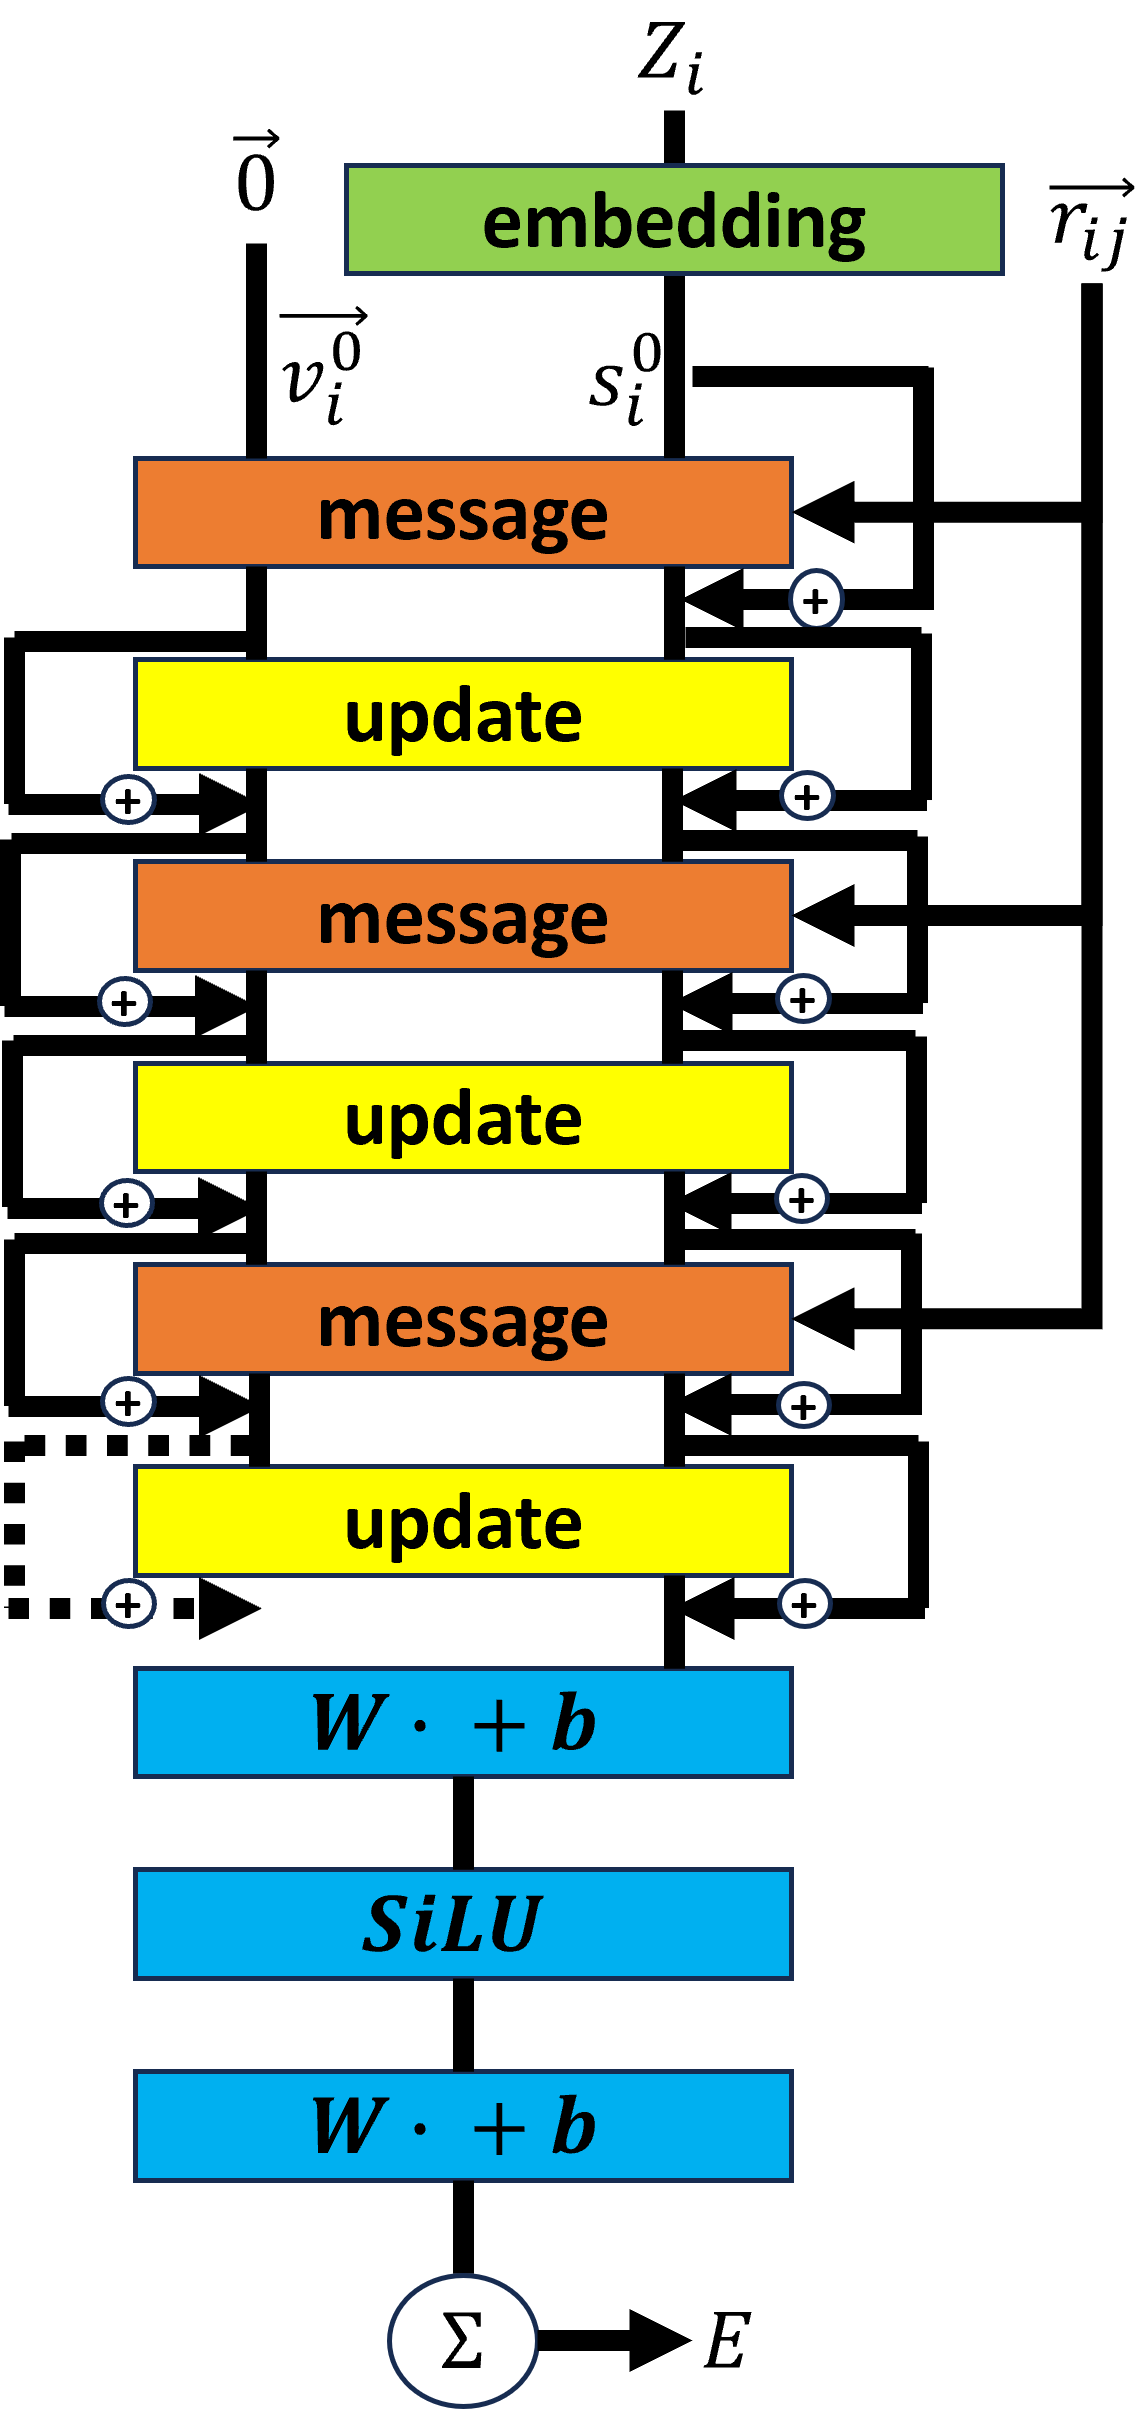
\includegraphics[width=150pt]{Images/Method/MPNN_arc.png}
\end{figure}

Worth noting about the full architecture, is the number of coupled message- and update-blocks, which is three. The output of these three
coupled sections will take the invariant scalar representations as input for a final set of layers, similar to the $\phi$-structure
presented earlier. Denote the scalar representations $\mathbf{s}_{i} \in \mathbb{R}^{F \times 1}$, the feature dimension $F$, utilizing the linear-layer-\ref{eq:linear_layer} and
SiLU\ref{eq:SiLU}-expressions from earlier. The expression of the output layer $O$ is then:

\begin{equation}
    \hat{\mathbf{y}} = \sum_{F} O(f_{6}(SiLU(f_{7}(\mathbf{s})))
\end{equation}

Which produces a set of predicted energies, which will be the output of the model. These output energies $\hat{\mathbf{y}}$, will be
compared to the targets of the model $\mathbf{y}$ to calculate the loss, via the mean squared error:

\begin{equation}\label{eq:loss}
    L = \frac{1}{N} \sum_{i=1}^N \left ( \hat{\mathbf{y}}_i - \mathbf{y}_i \right )^2
\end{equation}

This concludes the theoretical walkthrough of the inner workings of the implemented MPNN. The next section will detail the combination
of individual model architectures, into a bigger whole, namely an ensemble.

\subsection{Ensembles}

Ensembles (or Ensembling) is a technique for combining the predictive performance of individual modelling approaches
and to as an extension measuring uncertainty in the model. For the purpose of this study, only epistemic uncertainty, can be measured
in the models.

%#TODO MÅSKE: lav en figur der viser modeller som kombineres osv
In the context of MPNNs, ensembles can be created by training multiple models, in our case, on the same data set, 
with different initializations,
and combining their predictions to produce a mean and a variance among other metrics.
%#TODO Skriv noget mere her, omkring achored ensembles

\subsubsection{Descriptive statistics of the Ensemble}

Let $\mathbf{y}_i$ be the target binding energy for molecule $i$. Denote an ensemble of $T$ models where $t$ denotes a single model in the ensemble,
where $t \in \{1,2,\ldots,T\}$.
The ensemble prediction $\tilde{\mathbf{y}}_i$ can be calculated as the mean of the individual
model predictions $\mathbf{y}_{i,t}$, as done in\cite{Tran2019}, and proposed in \cite{Scalia2019}:

\begin{equation}\label{eq:mean-ensemble}
    \tilde{\mathbf{y}}_{i} = \frac{1}{T} \sum_{t=1}^{T} \mathbf{y}_{i,t}
\end{equation}

Further, in order to estimate the epistemic uncertainty in the ensemble predictions, we can calculate the variance based on individual model
predictions\cite{Tran2019}:

\begin{equation}\label{eq:variance-ensemble}
    \text{Var}(\mathbf{y}_{i}) = \frac{1}{T} \sum_{t=1}^T (\mathbf{y}_{i,t} - \tilde{\mathbf{y}}_i)^2
\end{equation}

\subsubsection{Uncertainty estimation}

Finally as the foundation of estimating uncertainty in the ensemble predictions, we can estimate the expected normal calibration error (ENCE).
This method relies on sorting metrics, in $K$ equal sized bins, where $k \in \{1,2,\ldots,K\}$ denotes a single bin.
A formal defintion of a bin is given below:
\begin{equation}\label{eq:bin}
    bin(x) = \begin{cases}
        1, & \text{if } x \text{ falls within the bin range} \\
        0, & \text{otherwise}
    \end{cases}
\end{equation}

Effectively outputting a result within a binary range, whether a given value, is within the bin range $1$, or outside the bin range $0$.

Further, we need to define a bin range. The bin ranges chosen are based on quantiles, which effectively will produce $K$ bins, of equal size.

Given a set of ascendingly sorted numbers $X = \{x_1, x_2, ..., x_n\}$ with $n$ elements. Denote a set of quantiles $P = \{p_0, p_1, ..., p_K\}$ with $K$ elements.
These quantiles are fractions of the number of elements in $X$ namely $n$ and the index $k$ of the element in $P$, specifically $\frac{p_{k}}{n}$.
The $p_{k}$-quantile of $X$, denoted as $Q(p_{k})$, is defined as follows:

\begin{itemize}
    \item Calculate the index of the quantile $q = p_{k} \cdot (n-1)$.
    \item If $q$ is an integer, $Q(p_{k})$ is equal to the $q$-th element of $X$, namely $x_{q}$.
    \item If $q$ is not an integer, $Q(p_{k})$ is equal to $\frac{1}{2} \cdot (x_{\lfloor q \rfloor} + x_{\lceil q \rceil})$
\end{itemize}

In the above, $\lceil \cdot \rceil$ and $\lfloor \cdot \rfloor$ denotes the ceiling and flooring functions respectively.
The ceiling function, denoted as $\lceil x \rceil$, rounds a real number $x$ up to the nearest integer greater than or equal to $x$. The flooring
function on the opposite, denoted as $\lfloor x \rfloor$, rounds a real number $x$ down to the nearest integer less than or equal to $x$.

These quantiles are then used to calculate the bin ranges:
\begin{equation}\label{eq:binrange}
    binrange(k) = \left[ Q(p_{k}); Q(p_{k+1}) \right]
\end{equation}

So for the final definition of the bin, utlizing the quantiles to produce bin ranges.

\begin{equation}\label{eq:bin-k}
    bin_{k}(x) = \begin{cases}
        1, & \text{if } x \in binrange(k) \\
        0, & \text{otherwise}
    \end{cases}
\end{equation}

Utilizing the above definition of a bin, we now want to sort all errors made by the individual models $e = y_{i} - {y}_{i,t}$ in ascending fashion.
We now define $K = \{1,2,\ldots,K\}$ bins, and $P = \{p_0, p_1, ..., p_K\}$ quantiles for the error metric to be sorted into bins.
the sorting is done via the below expression for all $k \in \{1,2,\ldots,K\}$ and all models $t \in \{1,2,\ldots,T\}$:

\begin{equation}\label{eq:bin-error}
    bin_{k}(e) =\begin{cases}
        1, & \text{if } e \in binrange(k) \\
        0, & \text{otherwise}
    \end{cases}
\end{equation}

We now wish to calculate the root mean squared error (RMSE) on each bin. The RMSE metric, describes the mean of empirical error, made
by all the models in the given bin. 
Denote the number of elements in the bin as $N$, where the
expression of the RMSE, is as follows:

\begin{equation}
    RMSE_{k} = \sqrt{\frac{1}{N} \sum_{n=1}^N \left( e_{n}^{(k)} \right)^2}
\end{equation}

We now go through a similar process, for variances over individual predictions and the means of the predictions 
$\text{Var}(\mathbf{y}_{i}) = \frac{1}{T} \sum_{t=1}^T (\mathbf{y}_{i,t} - \tilde{\mathbf{y}}_i)^2$. 
We sort them in ascending order. Define $K = \{1,2,\ldots,K\}$ bins, and $P = \{p_0, p_1, ..., p_K\}$ 
quantiles for the difference metric to be sorted into. the sorting is done via the below expression for all $k \in \{1,2,\ldots,K\}$ 
and all models $t \in \{1,2,\ldots,T\}$:

\begin{equation}\label{eq:bin-difference}
    bin_{k}(\text{Var}(\mathbf{y}_{i})) =\begin{cases}
        1, & \text{if } \text{Var}(\mathbf{y}_{i}) \in binrange(k) \\
        0, & \text{otherwise}
    \end{cases}
\end{equation}

Now wanting to produce the root mean variance (RMV) on each bin. The RMV metric, describes the variance on predictions, made
by all the models in the given bin.
Denote the number of elements in the bin as $N$, where the
expression of the RMV, is as follows:

\begin{equation}
    RMV_{k} = \sqrt{\frac{1}{N} \sum_{n=1}^N  \text{Var}(\mathbf{y}_{i})_{n}^{(k)}}
\end{equation}

We now wish to produce the ENCE-metric\ref{eq:calibration-error}\cite{Busk2021}.
This metric is produced based on the RMSE and RMV metrics, calculated further above.
These metrics are calculated for each $k$-bin, for the chosen number of bins $K$. The ENCE metric
is defined below, followed by the RMSE and the RMV.

\begin{equation}\label{eq:calibration-error}
    ENCE = \frac{1}{K} \sum_{k=1}^K \frac{|RMV_{k} - RMSE_{k}|}{RMV_{k}}
\end{equation}

These methods are heavily inspired by the methods in the papers\cite{Tran2019} and \cite{Busk2021}. Elements and approaches have been 
drawn from both, effectively doing cherrypicking for the scope of this project. The approach by Busk2021, is on models with two output
metrics, compared to this projects one. The paper by Tran2019, utilizes a similar approach to describing epistemic uncertainty in the
ensemble predictions, made by models with one output metric. But tran2019, lacks in the descriptive metrics that Busk2021 has, i.e 
RMSE, RMV, and ENCE.


\newpage
\section{Methods}\label{sec:methods}

This section will detail the implementation and necessary technological foundation, for applying the theories described,
in order to produce the experimental results for answering the research question. The section will also detail the necessary information,
for reproducing and understading the experimental results and their becoming.

\subsection{Experimental Setup}\label{subsec:setup}
The experimental setup are comprised of the following components:
\begin{itemize}
    \item Dataset
    \item Model
    \item Training- and Validation-Loop
    \item Test loop
\end{itemize}

These four components all together make up the main functionality of the experiment, and will be detailed individually
below. The detailing will have its focus on how concepts and theories previously explained,
are formatted and shaped, in order to be viable for practical modelling purposes.

\subsection{Dataset}\label{subsec:dataset}
The data set is comprised of one row for each node for 695 molecules, with a the following fields for each node:
\begin{itemize}
    \item Atom-type
    \item Overall binding energy (target property)
    \item x-coordinate
    \item y-coordinate
    \item z-coordinate
    \item Graph id
\end{itemize}
The atom type signifies the type of atom for a given node by name. The overall binding energy is the target property, for the full catalyst
process. This means all nodes with identical graph id will have a identical overall binding energy. The x, y, and z coordinates are the coordinates
of the nodes in the molecular graph, measured in Ångstrøm.

These fields are then translated to the relevant datastructures, via the graph data set constructor. This constructor
defines the following data structures, for utilization in the modelling task. Important to say is that the data set constructor,
constructs a data set of popentially several graphs, and not only one. The data set consists of the following critical fields:
\begin{itemize}
    \item num\_nodes: Number of nodes in the data set of graphs
    \item node\_from: The node from which the edge originates
    \item node\_to: The node to which the edge points
    \item num\_graphs: Number of graphs in the data set
    \item node\_graph\_index: The index of the graph the edge resides in
    \item unique\_atoms: The number of unique atoms in the data set
    \item edge\_lengths: The lengths of the edges
    \item edge\_vector\_diffs: The vector differences of the edges
\end{itemize}

The number of nodes in dataset, allows for the model to create initial state representation structures with proper dimensions for the
modelling task. The node\_from property, allows for summation of all neighbouring node state representations, within the cutoff limit,
into the designated node, we are trying to model in the message block. The node\_to property, allows for initialising the state representation
of the node in the update block, namely the scalar properties and the vector properties. The scalar properties are concatenated tensors of
embedded atom representations, linked by the index in the node\_to property. For scalar properties it is zero-vectors, instead of embedded
tensors. The num\_graphs property is used to initalize the initial state representation of the graphs. The node\_graph\_index property
is an index linking an edge, to a corresponding graph. When summing over all neighbour nodes occur, the full message state representation of all
neighbours under the cutoff, is summed over the node\_graph\_index property, to produce a state representation of graphs. The unique\_atoms
property, allows for the embedding function to create a unique atom representation for each type of atom in the data set. The edge\_lengths
allow for a masking of the edges and thereby nodes that are not within the cutoff limit. The edge\_vector\_diffs are the vector differences
of the edges, being an input variable in the message block.



\subsection{Model}\label{subsec:model}

The model architecture consists of two main components, namely the Message block, and the Update block as formerly introduced in the
the theory section \ref{eq:message_block}, and \ref{eq:update_block}.  The Message block is conceptually responsible
for the message passing between the nodes in the graph, allowing for the flow of information between the nodes.
This information is then summed up and stored in state variables in the form of a scalar and vector representation.
This summation is done in a residual manner, following the implementation of the PAINN architecture\cite{PAINN}. An equation
defining the residual calculation of the scalar-properties\ref{eq:residual_scalar} and vector-properties\ref{eq:residual_vector}
can be found below, as well as an illustration of the message block\ref{img:message_block}.

\begin{equation}\label{eq:residual_scalar}
    \Delta \mathbf{s}_{i}^{m}= (\phi_{s}(\mathbf{s}) * \mathcal{W}_{s})_{i} = \sum_{j} \phi_{s}(\mathbf{s}) \circ \mathcal{W}_{s} \left ( \left \| r_{ij} \right \| \right )
\end{equation}

\begin{equation}\label{eq:residual_vector}
    \Delta \vec{\mathbf{v}}_{i}^{m}= \sum_{j} \vec{\mathbf{v}}_{j} \circ \phi_{vv}(\mathbf{s}_{j}) \circ \mathcal{W}_{vv} \left ( \left \| r_{ij} \right \| \right ) + \sum_{j} \phi_{vs}(\mathbf{s}_{j}) \circ \mathcal{W}'_{vs} \left ( \left \| r_{ij} \right \| \right ) * \frac{r_{ij}}{\left \| r_{ij} \right \|}
\end{equation}

\begin{figure}[H]
    \caption{Message Block}
    \centering\label{img:message_block}
    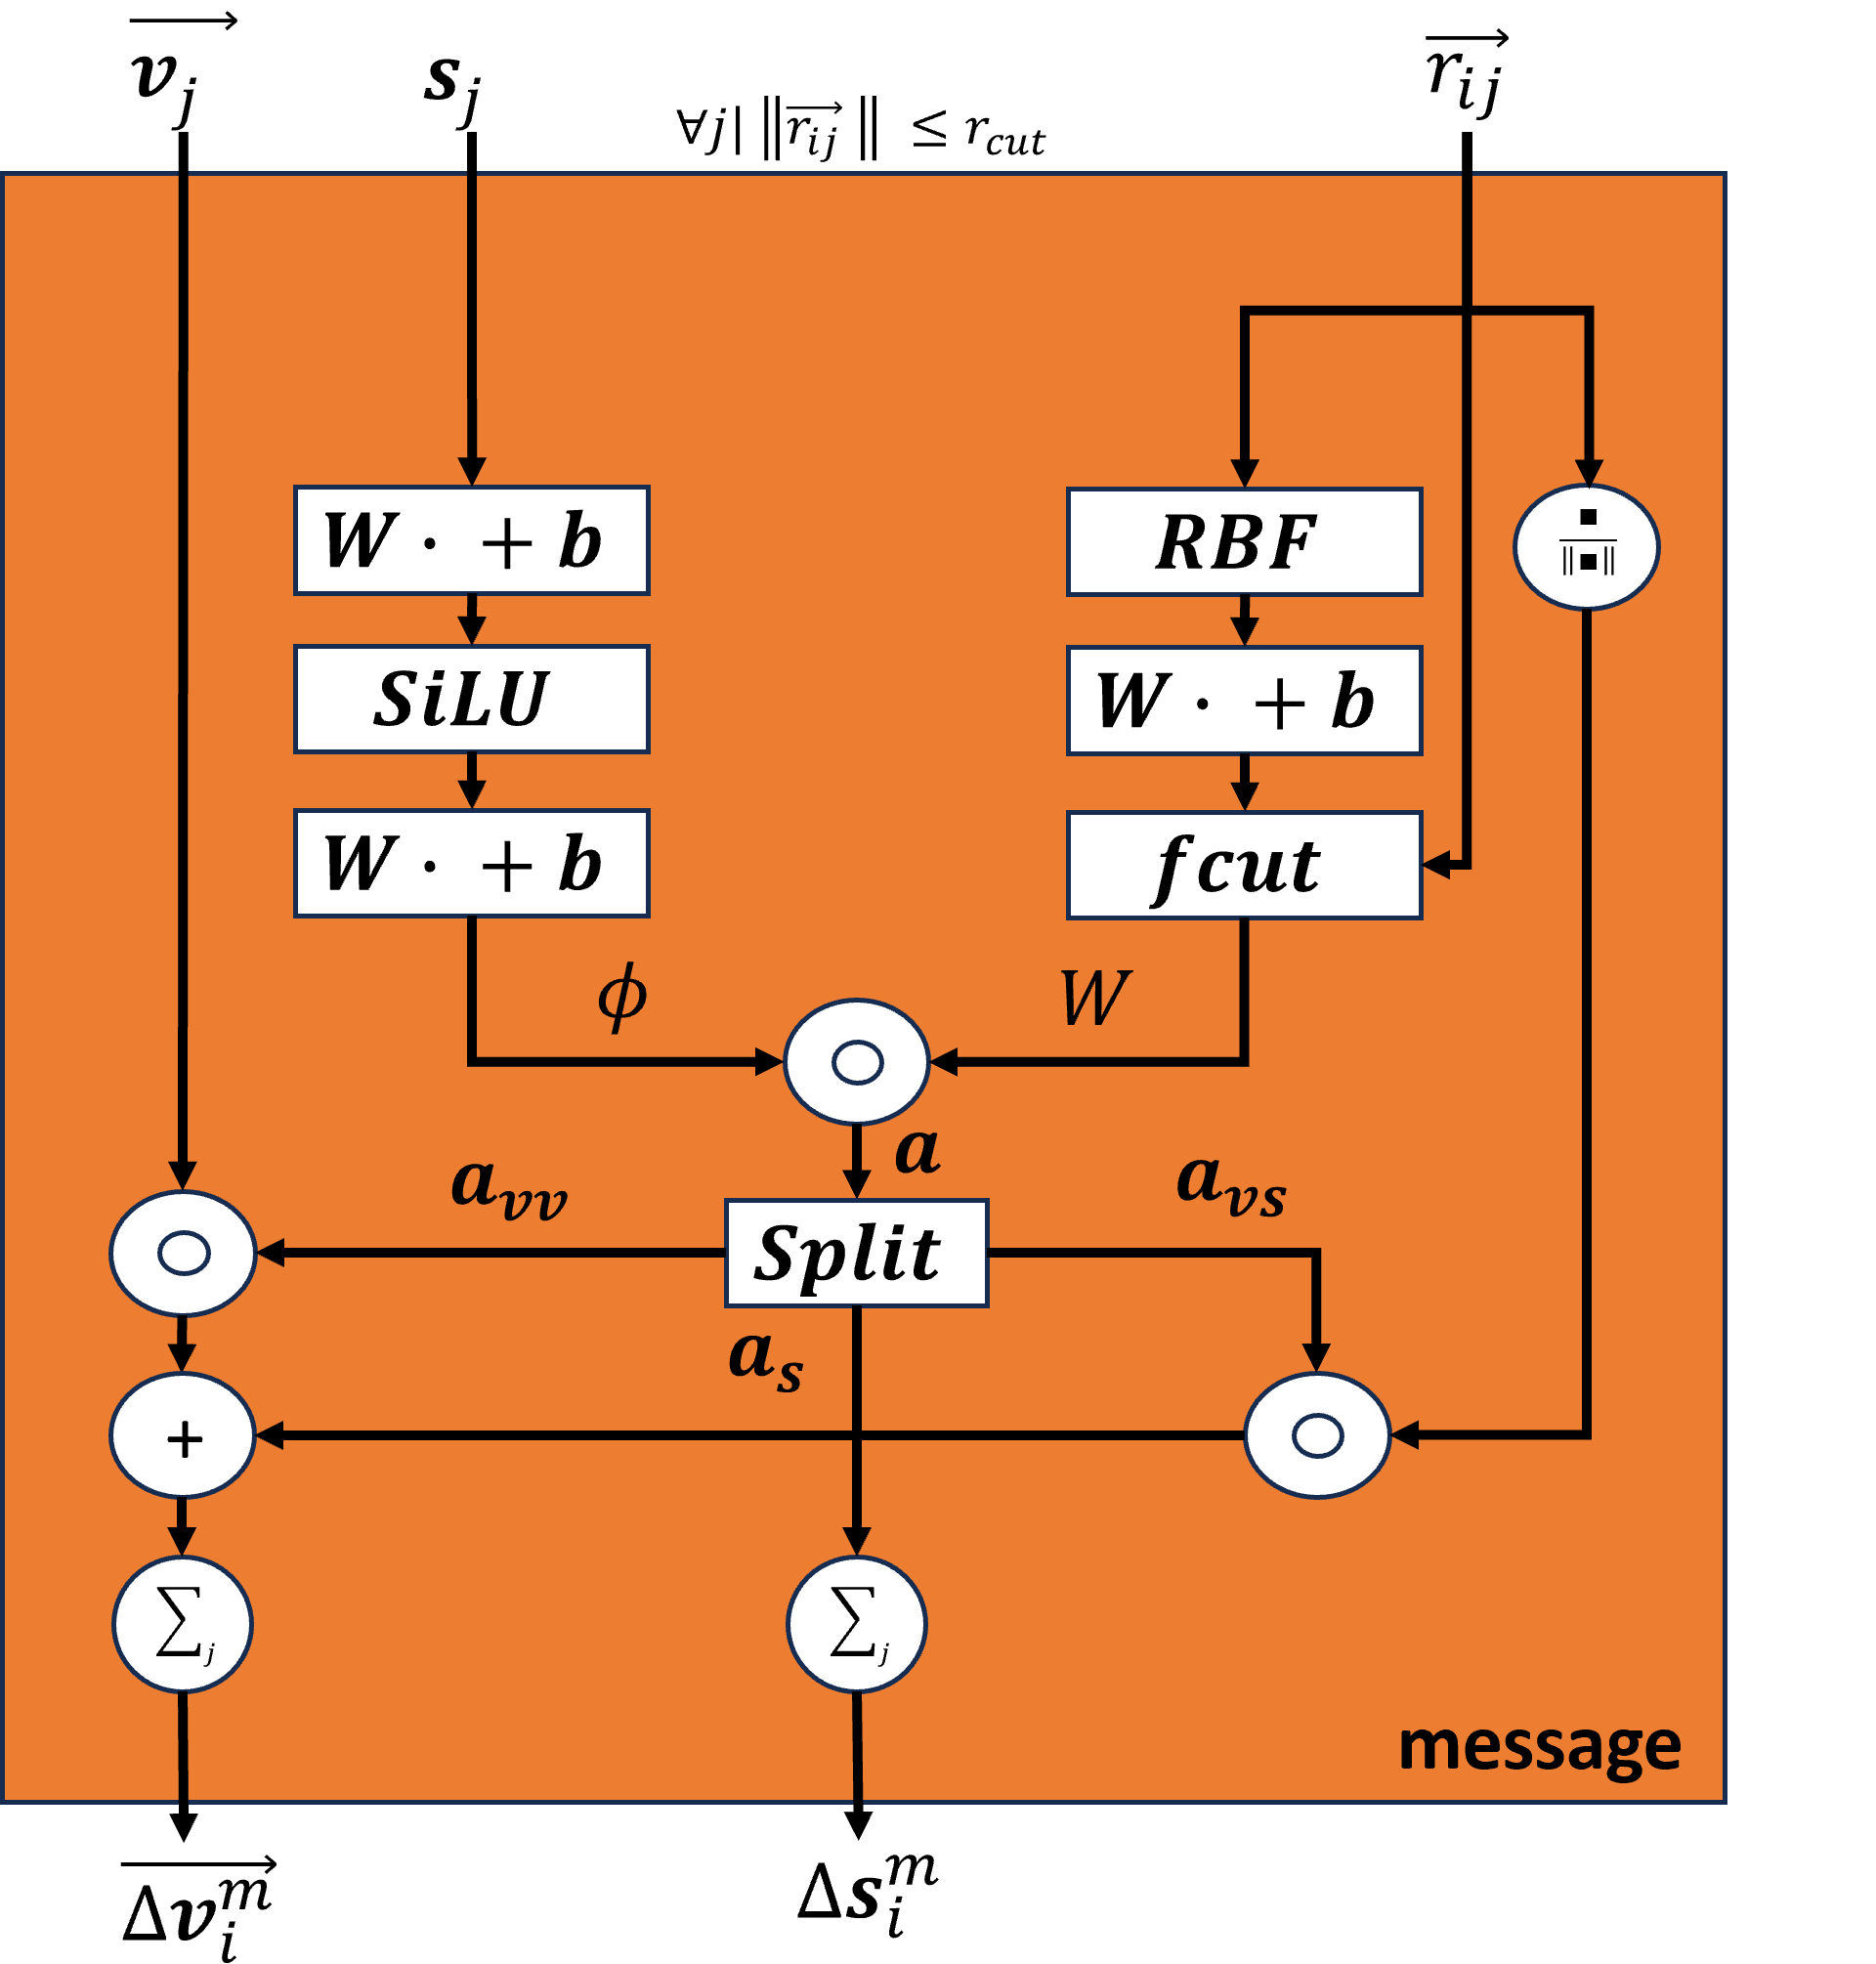
\includegraphics[width=250pt]{Images/Method/message_block.png}
\end{figure}

Worth noting about the figure, compared to the similar one in \cite{PAINN}, is the use of the \textit{r\_ij} vector, that also flow into
the 'fcut' function, as mentioned in \ref{subsec:modelling_task}. The model in this paper, does not highlight the dimension expansions
or collisions from network element to network element, due to the model parameters varying in size, as it is the scope of this project
to investigate similarities or dissimilarities in performance, with respect to the PAINN architecture and dissimilar state representation
sizes. both sizes $\phi$ and $\mathcal{W}$ are chosen sub-architectures based on the PAINN architecture from\cite{PAINN}. The image
also contains hints of the $\mathbf{a}$-tensor, which is a product of the $\phi$ and $\mathcal{W}$ tensors, and not highlighted in \cite{PAINN}.

The residual values produced in the message block, then used in the update block, in order to update the node states,
based on the summation over neighbouring states.
This structure is also heavily inspired by the PAINN architecture\cite{PAINN}. The below equations represent the residual updates
on both the scalar- \ref{eq:residual_scalar_update} and the vector- \ref{eq:residual_vector_update} properties. Below is also
a figure representing the update block\ref{img:update_block}.

\begin{equation}\label{eq:residual_scalar_update}
    \Delta \mathbf{s}_{i}^{u}= \mathbf{a}_{ss} \left ( \mathbf{s}_{i}, \left | \mathbf{V\vec{v}_{i}} \right | \right ) + \mathbf{a}_{sv} \left ( \mathbf{s}_{i}, \left | \mathbf{V\vec{v}_{i}} \right | \right ) \left \langle \mathbf{U\vec{v}_{i}}, \mathbf{V \vec{v}_{i}} \right \rangle
\end{equation}

\begin{equation}\label{eq:residual_vector_update}
    \Delta \mathbf{v}_{i}^{u}= \mathbf{a}_{vv} \left ( \mathbf{s}_{i}, \left | \mathbf{V\vec{v}_{i}} \right | \right ) \mathbf{U\vec{v}_{i}}
\end{equation}



The blocks are stacked in coupled sequences of five full rounds, like the illustration below highlights\ref{img:MPNN_arc}, a corresponsding model can be found
in \cite{PAINN}. The illustration shows an architecture comprised of three sets of message- and update-blocks, the implementation in this project utilized
five sets. The model representation property $\vec{v_i^{0}}$ is initialized to the zero vector, and the scalar property $S_{i}^{0}$
is initialized to a random embedding on atom level, for each node in the graph.


\begin{figure}[H]
    \caption{MPNN Full Architecture}
    \centering\label{img:MPNN_arc}
    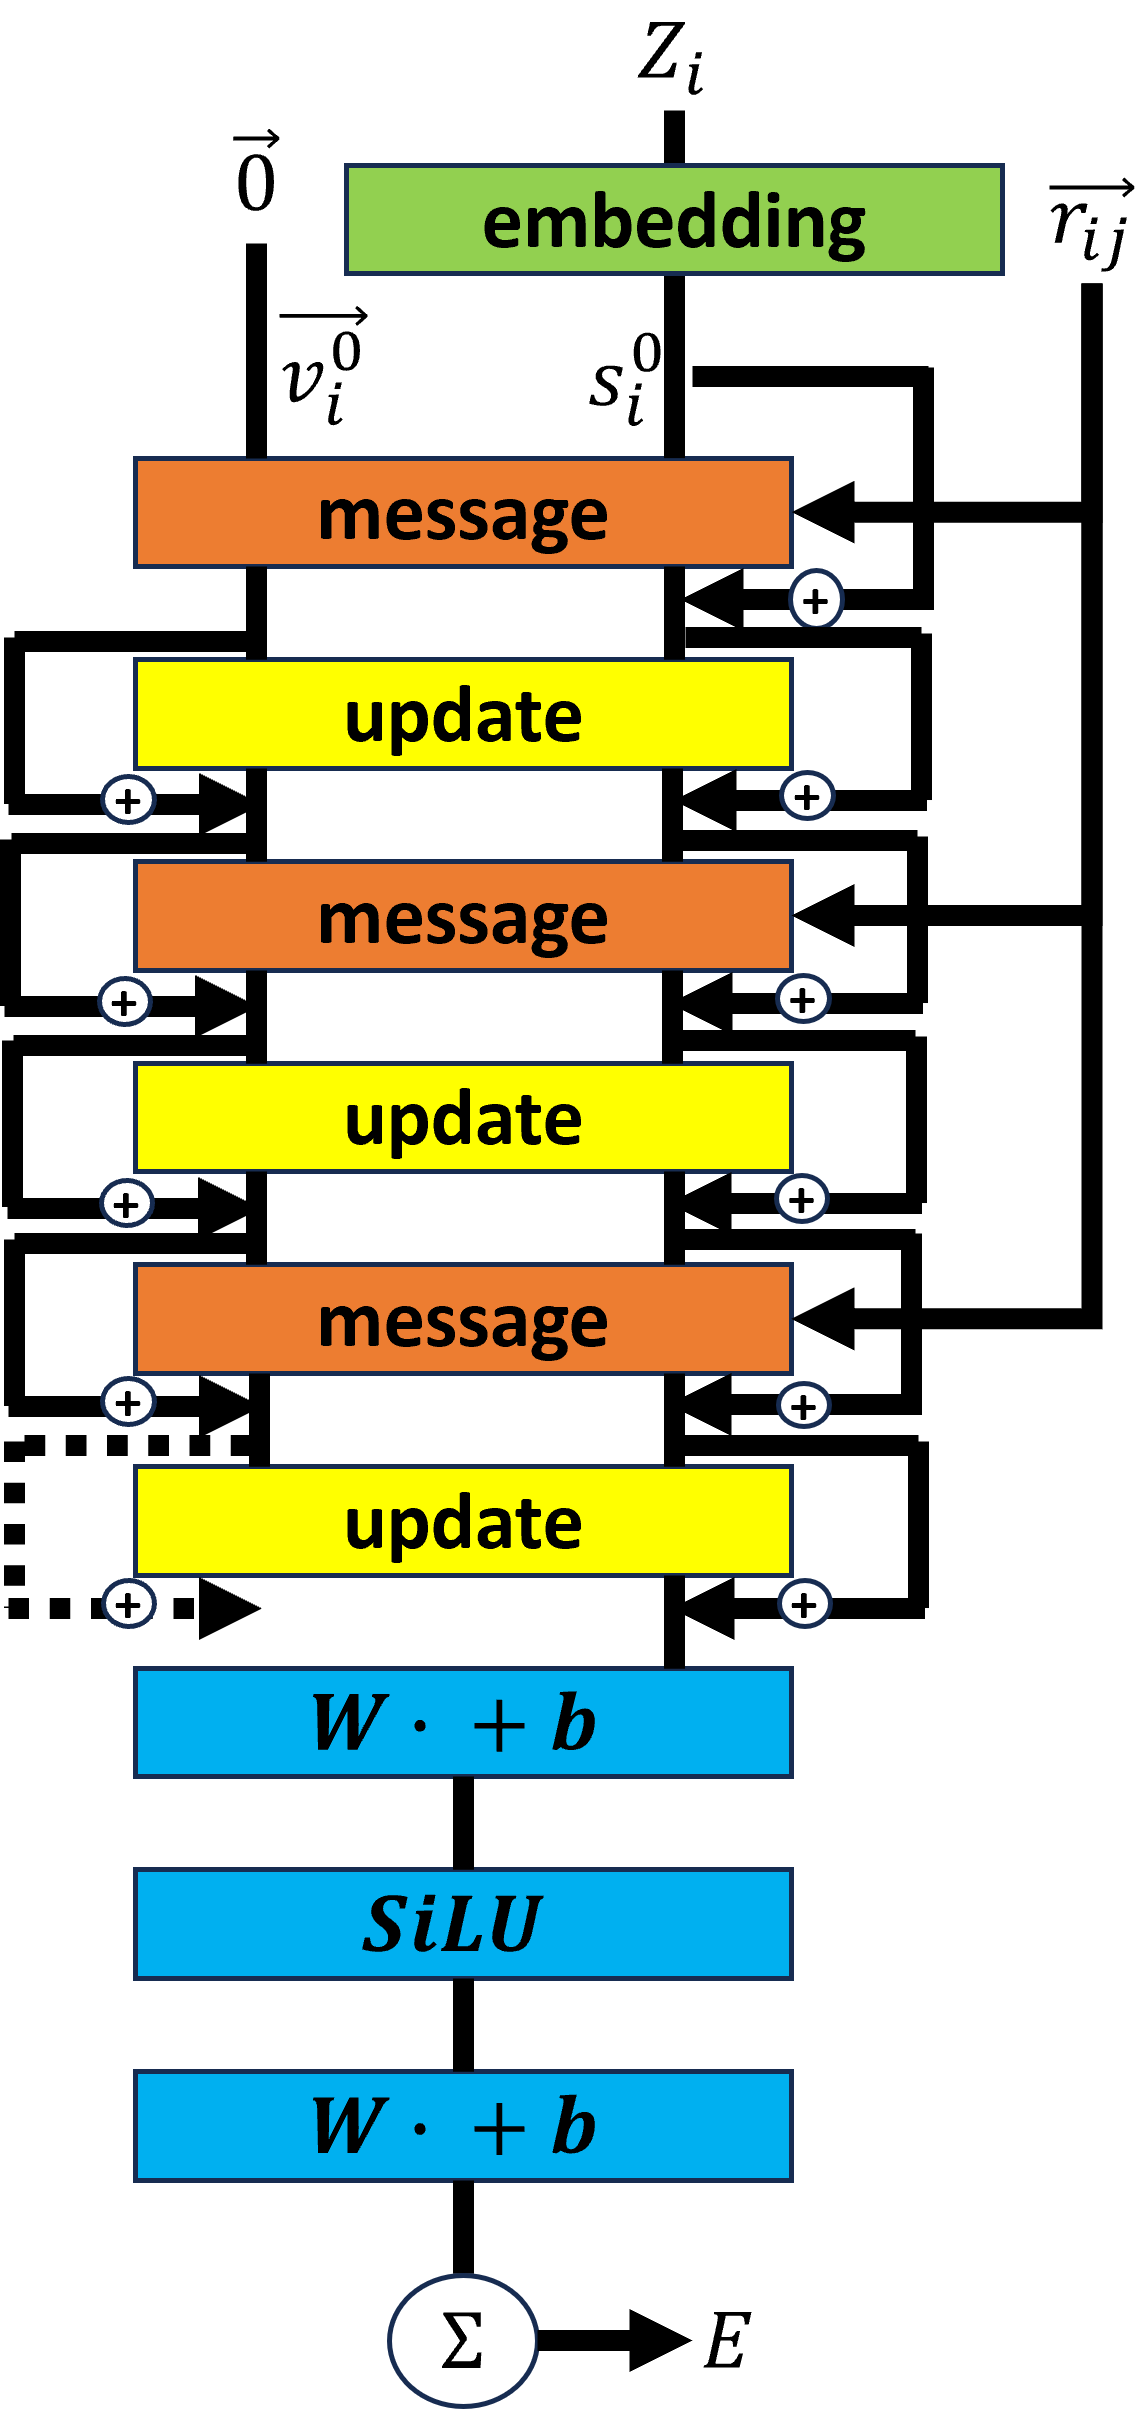
\includegraphics[width=200pt]{Images/Method/MPNN_arc.png}
\end{figure}

\subsection{Training- and Validation-loop}\label{subsec:training}

\begin{algorithm}[H]
    \begin{algorithmic}[1]
        \State Initialize size of ensemble: $T$
        \State Initialize size of batch: $B$
        \State Initialize data sets: $Td, Vd$
        \State initialize training data loader: $TD = Dataloader(B,Td)$
        \State initialize validation data loader: $VD = Dataloader(B,Vd)$
        \State Initialize number of epochs: $E$
        \State Initialize validation index: $V$

        \For {$model=1,2,\ldots, T$}

        \State Initialize MPNN model instance: $model = PAINN()$
        \State initialize MSE loss function: $loss = MSE()$
        \State Initialize Adam optimizer: $optimizer = Adam(model.parameters())$
        \State Initialize learning rate scheduler: $scheduler = StepLR(optimizer)$

        \For {$epoch=1,2,\ldots,E$}

        \For {$batch=1,2,\ldots,TD$}

        \State Normalize targets: $y = normalize(y)$
        \State Predict binding energy: $\hat{y} = model(batch)$
        \State Calculate loss: $l = loss(y,\hat{y})$
        \State Backward pass: $l.backward()$
        \State Optimizer step: $optimizer.step()$

        \If {$epoch \% V == 0$}
        \State Model in evaluation mode: $model.eval()$

        \For {$batch=1,2,\ldots,VD$}

        \State Normalize targets: $y = normalize(y)$
        \State Predict binding energy: $\hat{y} = model(batch)$
        \State Calculate loss: $l = loss(y,\hat{y})$
        \State Apply exponential smoothing: $l = l * 0.9 + l_{-1} * 0.1$
        \State Scheduler step: $scheduler.step(l)$
        \EndFor

        \EndIf
        \EndFor
        \EndFor
        \EndFor
    \end{algorithmic}
    \caption{MPNN Training Loop}
    \label{algo:MPNN_training}
\end{algorithm}

\subsection{Test Loop}\label{subsec:test}

\begin{algorithm}[H]
    \begin{algorithmic}[2]
        \State Initialize size of ensemble: $T$
        \State Initialize size of batch: $B$
        \State Initialize data sets: $Testd, $
        \State initialize training data loader: $TestD = Dataloader(B,Testd)$

        \For {$model=1,2,\ldots, T$}
        \State Initialize target list: $y_{l}$
        \State Initialize prediction list: $\hat{y}_{l}$
        \For {$batch=1,2,\ldots,TestD$}
        \State Normalize targets: $y = normalize(y)$
        \State Predict binding energy: $\hat{y} = model(batch)$
        \State Calculate loss: $l = loss(y,\hat{y})$
        \State Append target to list: $y_{l}$
        \State Append prediction to list: $\hat{y}_{l}$
        \EndFor
        \State Save predictions and targets to file
        \State Save model to file
        \EndFor
    \end{algorithmic}
    \caption{MPNN Testing Loop}
    \label{algo:MPNN_testing}
\end{algorithm}

\subsection{Modelling Hyperparameters}\label{subsec:mod-hyper}

Generally, two subsets of hyperparameters exists, those relevant to the less sophisticated set of ensemble models (titled MPNN64), and those
relevant to the more sophisticated ensemble models (titled MPNN128). The table below\ref{tab:hyperparameters},
details shared and non-shared model hyperparameters, as well
as highlighting the parameters, which are consistent with the PAINN architecture described in \cite{PAINN} with a star (*).

\begin{table}[H]
    \centering
    \caption{Modelling hyperparameters}
    \label{tab:hyperparameters}
    \begin{tabular}{|lcll|}
        \hline
        \multicolumn{1}{|l|}{\textbf{Model Hyperparameters}}                 & \multicolumn{1}{l|}{\textit{\textbf{MPNN64}}} & \multicolumn{1}{l|}{\textit{\textbf{MPNN128}}} & \textit{\textbf{Unit}} \\ \hline
        \multicolumn{4}{|c|}{\textbf{Shared}}                                                                                                                                                          \\ \hline
        \multicolumn{1}{|l|}{\textbf{Number of physical dimensions*}}        & \multicolumn{2}{c|}{3}                        & Dimensions                                                              \\ \hline
        \multicolumn{1}{|l|}{\textbf{Number of Message Passing Rounds*}}     & \multicolumn{2}{c|}{5}                        & Rounds                                                                  \\ \hline
        \multicolumn{1}{|l|}{\textbf{Patience*}}                             & \multicolumn{2}{c|}{5}                        & Validation steps                                                        \\ \hline
        \multicolumn{1}{|l|}{\textbf{Weight Decay*}}                         & \multicolumn{2}{c|}{0.01}                     & N/A                                                                     \\ \hline
        \multicolumn{1}{|l|}{\textbf{Learning Rate Decay*}}                  & \multicolumn{2}{c|}{0.5}                      & N/A                                                                     \\ \hline
        \multicolumn{1}{|l|}{\textbf{Exponential Smoothing for Validation*}} & \multicolumn{2}{c|}{0.9}                      & N/A                                                                     \\ \hline
        \multicolumn{1}{|l|}{\textbf{Radial Basis Parameter*}}               & \multicolumn{2}{c|}{20}                       & N/A                                                                     \\ \hline
        \multicolumn{1}{|l|}{\textbf{Learning Rate}}                         & \multicolumn{2}{c|}{0.001}                    & N/A                                                                     \\ \hline
        \multicolumn{1}{|l|}{\textbf{Cutoff Distance}}                       & \multicolumn{2}{c|}{4}                        & Ångstrøm                                                                \\ \hline
        \multicolumn{4}{|c|}{\textbf{Not shared}}                                                                                                                                                      \\ \hline
        \multicolumn{1}{|l|}{\textbf{State dimension size}}                  & \multicolumn{1}{c|}{64}                       & \multicolumn{1}{c|}{128}                       & Dimensions             \\ \hline
    \end{tabular}
\end{table}
%#TODO Indsæt link til appendix som forklarer de forskellige hyperparametre

An explanation of the individual hyperparameters influence on the model, and a justification for selection of the above values, can be
be found in the appendix section\ref{subsec:appendixA}.

\subsection{Experimental Hyperparameters}\label{subsec:experiement}

The experimental hyperparameters defining the implementation of the above model setting, can be found in
table below\ref{tab:experiment}.

\begin{table}[H]
    \centering
    \caption{Experimental Hyperparameters}
    \label{tab:experiment}
    \begin{tabular}{|l|c|c|}
        \hline
        \textbf{Experimental Hyperparameters}                          & \multicolumn{1}{l|}{\textit{\textbf{Value}}} & \textit{\textbf{Unit}} \\ \hline
        \multicolumn{1}{|c|}{\textbf{Number of molecules in Data Set}} & 695                                          & Molecules              \\ \hline
        \textbf{Training Split}                                        & 0.8                                          & N/A                    \\ \hline
        \textbf{Validation Split}                                      & 0.1                                          & N/A                    \\ \hline
        \textbf{Test Split}                                            & 0.1                                          & N/A                    \\ \hline
        \textbf{Ensemble Size}                                         & 5                                            & Models                 \\ \hline
        \textbf{Initial number of Epochs}                              & 200                                          & Epochs                 \\ \hline
        \textbf{Validation Index}                                      & 5                                            & Epochs                 \\ \hline
        \textbf{Model Saving Interval}                                 & 0.01                                         & N/A                    \\ \hline
        \textbf{Batch Size}                                            & 5                                            & Molecules              \\ \hline
    \end{tabular}
\end{table}

An in explanation of the selection of experiment hyperparameters and justification,
be found in the appendix section\ref{subsec:appendixB}.

\subsection{Software tools and Hardware}\label{subsec:software}

The projects execution were developed in Python 3.10.9, with heavy emphasis on Pytorch, Numpy and Pandas,
supported by few shell scripts for cloud job definitions.
A full list of packages, and their versions utilized in the experiment, can be seen in appendix\ref{subsec:appendixC}
The initial datastructures and pipeline were inspired by course-material made by Mikkel Nørgaard Schmidt.
The hardware utilized for the final experimental setup, were two two types of GPUs, belonging
to the High Performance Computing (HPC) cluster at the Technical University of Denmark (DTU).
The two queues utilized were 'gpua100' and 'gpuv100'. For further details on the hardware,
please refer to the following reference:\cite{hpc}. Total computation time in the cloud was three days,
in order to produce the trained ensemble of ten individual models.

\subsection{Reproduceability}\label{subsec:reproduceability}

For reviewing and reproduceability purposes,
the following github link stores the latest version of the code: \url{https://github.com/Lohmann94/head},
which was utilized in the experiment. The experiment can be reproduced with the following seed-values\ref{tab:seeds},
which can be found for individual models:

\begin{table}[H]
    \centering
    \caption{Model seeds for reproduction}
    \label{tab:seeds}
    \begin{tabular}{|cc|cc|}
        \hline
        \multicolumn{2}{|c|}{\textbf{MPNN128 Ensemble:}} & \multicolumn{2}{c|}{\textbf{MPNN64 Ensemble:}}                                                                         \\ \hline
        \multicolumn{1}{|c|}{\textit{\textbf{Model}}}    & \textit{\textbf{Seed}}                         & \multicolumn{1}{c|}{\textit{\textbf{Model}}} & \textit{\textbf{Seed}} \\ \hline
        \multicolumn{1}{|c|}{\textbf{MPNN128\_1}}        & 49                                             & \multicolumn{1}{c|}{\textbf{MPNN64\_1}}      & 90                     \\ \hline
        \multicolumn{1}{|c|}{\textbf{MPNN128\_2}}        & 10                                             & \multicolumn{1}{c|}{\textbf{MPNN64\_2}}      & 52                     \\ \hline
        \multicolumn{1}{|c|}{\textbf{MPNN128\_3}}        & 100                                            & \multicolumn{1}{c|}{\textbf{MPNN64\_3}}      & 7                      \\ \hline
        \multicolumn{1}{|c|}{\textbf{MPNN128\_4}}        & 20                                             & \multicolumn{1}{c|}{\textbf{MPNN64\_4}}      & 9                      \\ \hline
        \multicolumn{1}{|c|}{\textbf{MPNN128\_5}}        & 30                                             & \multicolumn{1}{c|}{\textbf{MPNN64\_5}}      & 87                     \\ \hline
    \end{tabular}
\end{table}

The cloud-job configuration variables for reproducing with the described performance,
can be found in the below table\ref{tab:cloud-job-param}:

\begin{table}[]
    \centering
    \caption{Cloud Job Parameters}
    \label{tab:cloud-job-param}
    \begin{tabular}{|c|c|c|}
        \hline
        \textbf{Cloud Job Parameters} & \textit{\textbf{MPNN128}} & \textit{\textbf{MPNN64}}              \\ \hline
        \textbf{Queue}                & \textbf{gpuv100}          & \multicolumn{1}{l|}{\textbf{gpua100}} \\ \hline
        \textbf{Number of cores}      & 8                         & 8                                     \\ \hline
        \textbf{Memory/Cores}         & 5 gb                      & 5 gb                                  \\ \hline
        \textbf{Number of hosts}      & 1                         & 1                                     \\ \hline
    \end{tabular}
\end{table}

\newpage

\section{Data}\label{sec:data}

\subsection{Cross Coupling Catalysts}

The data set of interest consists of 7.054 optimized geometries of compounds being candidate structures in oxidative addition 
catalystic process. The optimized geometries will have a binding energy associated with it, that dictates the net energy 
produced by the oxidative addition of a specific transition metal\cite{Meyer2018}, which is the target of our modelling task. 
The original papers set out to further select 557 catalyst candidates which are within a predefined thermodynamic window, and a 
further selection of candidates based on their pricepoint per mol.\\

The molecular compounds are represented as graph structures of nodes and edges. The nodes constitute atoms, and the edges molecular 
connections between atoms. The representation will further consist of Cartesian coordinates provided in the data set, fixing the 
individual nodes in three dimensional space. This also provides the data set with the possibility of deriving distances between the 
nodes, or the length of edges, which are crucial to the modelling efforts.\\ 

The number of number of nodes in the graphs, range from a minimum of 5, a mean of 52.51, to a maximum of 123 nodes. 
A bar plot of the number of graphs in various buckets of node-counts, can be seen below\ref{num_nodes}.\\

\begin{figure}[H]
\caption{Bar plot of number of nodes per graph}
\centering\label{num_nodes}
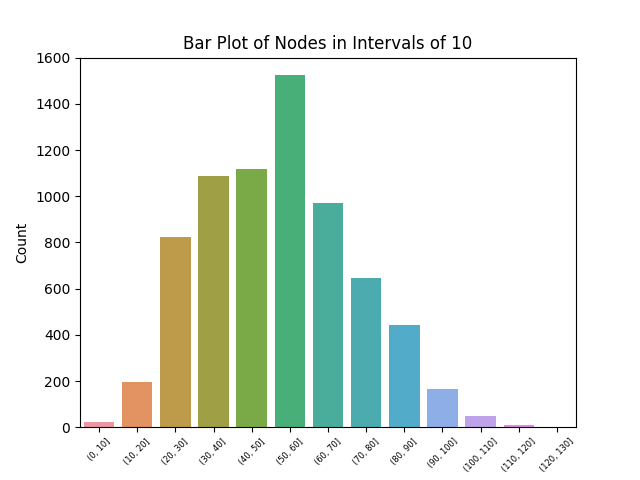
\includegraphics[width=\textwidth]{Images/Data/num_nodes_dataset.png}
\end{figure}

The atom distribution of the graphs a constituted by 13 unique atoms being:
 \begin{itemize}  
 \item H: Hydrogen  
 \item C: Carbon  
 \item N: Nitrogen  
 \item P: Phosphorus  
 \item O: Oxygen  
 \item Cl: Chlorine  
 \item Pd: Palladium  
 \item F: Fluorine  
 \item Au: Gold  
 \item Cu: Copper  
 \item Ag: Silver  
 \item Pt: Platinum  
 \item Ni: Nickel 
 \end{itemize}

The distribution of the above atoms, can be seen in a Pareto graph below\ref{pareto_atoms}. 
The distribution is mainly made up by hydrogen and carbon, those two being 90.6 percent of the atom-representation combined. 
The next highest contributor is nitrogen, only representing 3,4 percent of the atoms. 
The remaining atoms constitute 6 percent of the atom representation in the data set.

\begin{figure}[H]
\caption{Pareto plot of atom distribution in data set}
\centering\label{pareto_atoms}
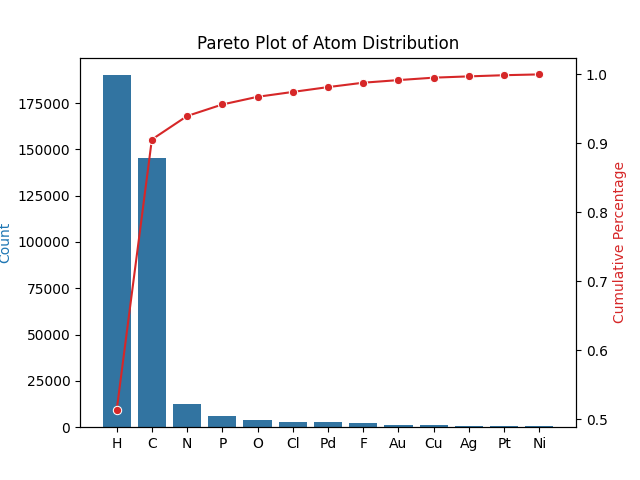
\includegraphics[width=\textwidth]{Images/Data/pareto_atom_distribution.png}
\end{figure}

The additive part of the catalyst process, are selected transition metals, namely: 

\begin{itemize}
  \item Pd: Palladium
  \item Au: Gold
  \item Cu: Copper
  \item Ag: Silver
  \item Pt: Platinum
  \item Ni: Nickel
\end{itemize}

The data set consists of the following distribution of the above transition metals, below can be seen a pareto similar to further above, 
but now show the distribution of transition metals in the data set\ref{addition_atoms}.

\begin{figure}[H]
\caption{Pareto plot of transition metal distribution in data set}
\centering\label{addition_atoms}
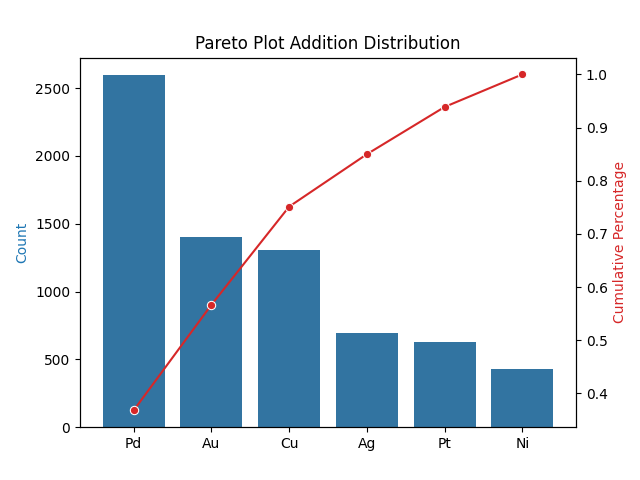
\includegraphics[width=\textwidth]{Images/Data/addition_distribution.png}
\end{figure}

The distribution is mainly comprised of Palladium and Gold, standing for 57 percent of the transition metals in the data set. \\

The catalyst process can be both exothermic and endothermic, represented in either a positive net binding energy as a target, 
or a negative net binding energy as a target for the regression task. The regression targets range from a minimum of -80.82 
being endothermic, to 61.49 being exothermic, where the mean is placed at -18.62. A bar plot with buckets of ten,
 of the distribution of targets can be seen below\ref{binding_energies}.

\begin{figure}[H]
\caption{Bar plot of binding energy distribution in targets}
\centering\label{binding_energies}
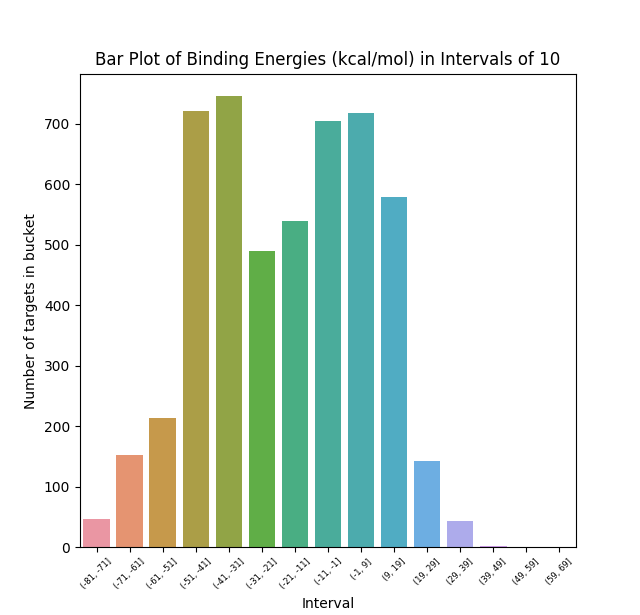
\includegraphics[width=\textwidth]{Images/Data/binding_energies.png}
\end{figure}

The edge-wise distances between nodes, measured in ångstrom, are crucial to the modelling task, since a model-parameter called `r-cut', 
defines a cutoff limit from which edges with a distance lower than the cutoff are defined as neighbours of a given node, and those above 
as non-neighbours. The neighbours goes are allowed a higher model influence, and therefore understanding where to set the cutoff, 
is a crucial hyperparameter. The distances of the full data set is intractable to compute locally, so a subset of 50 randomly chosen 
graphs and their edge-wise distances are plotted as a representation of the full data set\ref{distances}. As we can see in the plot, 
most distances are covered by the interval 0 to 7, at 64 percent, and only 20 percent of distances lie in the interval above 8.5. \\

\begin{figure}[H]
\caption{Pareto plot of Distances between edges from 50 graphs}
\centering\label{distances}
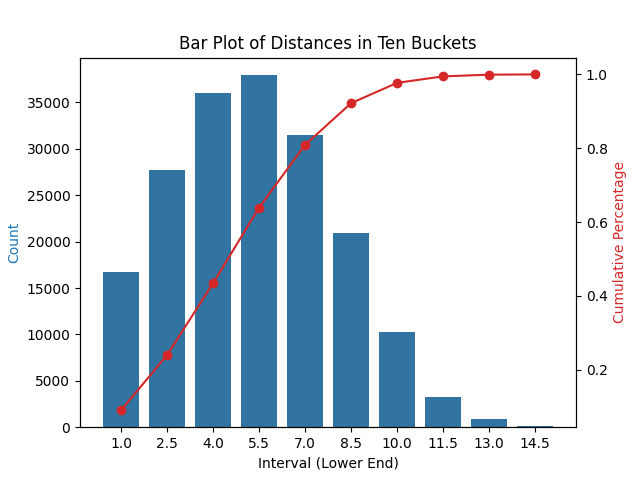
\includegraphics[width=\textwidth]{Images/Data/distances.png}
\end{figure}

In a chemistry context, it is argued that a large portion in the variance in binding energy, can be explained by local interactions 
among atoms\cite{PAINN}. So even though a high degree of information lies beyond cutoff limits of i.e four or five, then information 
might not be crucial to the prediction in energy we are trying to make. \\

The modelling task will take in a given molecular structure, and produce a regression metric, trying to predict the associated 
binding energy from the oxidative addition in the unit kcal/mol. Further more, the regression efforts will be put in an ensemble 
context of a number of structurally similar models, producing a mean and a variance over the predicted regression metric from the 
ensemble.\\

\subsection{Data Privacy- and Quality-issues}

Due to the data sources being publicly available for download, under the creative commons attribution 4.0 license,
 the implementation and storage of the data, has been chosen to support all project activities in the most convenient way. 
 Specifically that mean local and cloud storage, without password protection or encryption of the raw data. \\

The field of chemistry, that this study supports computationally, 
provide research which are used within the life-science industry for drug-discovery among other fields. \\

With this in mind, sourcing of the data set needs to be carefully handled, 
taking into account potential end-user risks of promoting various molecules and processes through research, 
at some point in the process before consumption. The sourcing of the Cross-Coupling data set, is partly transparent. 
The initial data set is comprised of 25.116 graph structures, and was sourced through generating options based on 6 transition metals, 
mentioned above, and 91 ligands. This generation process was made by combining all possible combinations of the six transition metals 
and the 91 ligands, applying a filter for redundant chemical properties to reach the initial 25.116 size data set\cite{Meyer2018}. 
The reduction in data set size to the 7.054, was done by training a model to predict a chemical descriptor value relating to certain 
energy-levels, and then selecting these 7.054 molecules and transition metals based on that. No apparent precaution towards end-user 
complications are mentioned, and should therefore be applied further down stream of the research efforts within this field. 

\newpage


\section{Results}\label{sec:results}

%#TODO plot RMV and RMSE against each other like busk2021

%#TODO husk at kommentere på epistemisk usikkerhed, forbundet med grafer og metriker

%#TODO test_loss_128 mean: 36.799533534049985, testloss_64 mean: 37.081851065158844

%#TODO gennemsnitlig varians over ensemble i testsets for 64: 0.29809390719701073 og for 128: 0.15309279243460014

%#TODO ence for MPNN64 ensemble: 23.50 , 128: 32.06

%# ensemble vs. single models() first ensemble model); 64: [0.969972792480524, 0.9676276973022239, 0.9888736279961788, 0.9828243429827256, 0.9988442451349356, 1.2097879561835665], 128: [0.9900557188310352, 1.0342352502056764, 1.017243472314507, 1.0004067356869728, 1.0409579224317915, 1.0105280059508281]

%#TODO sammenlign MSE for ensemble64: 0.96 og ensemble128: 0.99

%#TODO nævn noget med at training loss og val loss data kun gemmes med lav frekvens, derfor er der sammenfald på mange af batch længderne
%#TODO nævn noget med at early stopping blev triggered, men ikke stoppede før den fulde epoch var færdig. derfor kommer både loss og number of gradient steps i intervaller af 315


\begin{table}[H]
    \centering
    \caption{Number of gradient steps, for individual models in ensembles}
    \label{tab:num-steps}
    \begin{tabular}{|cccc|}
    \hline
    \multicolumn{4}{|c|}{\textbf{MPNN ensembles total gradient steps}}                                                                         \\ \hline
    \multicolumn{2}{|c|}{\textit{\textbf{MPNN128 Ensemble}}}                        & \multicolumn{2}{c|}{\textit{\textbf{MPNN64 Ensemble}}}   \\ \hline
    \multicolumn{1}{|c|}{\textbf{Model}}      & \multicolumn{1}{c|}{\textit{Value}} & \multicolumn{1}{c|}{\textbf{Model}}     & \textit{Value} \\ \hline
    \multicolumn{1}{|c|}{\textbf{MPNN128\_1}} & \multicolumn{1}{c|}{630}            & \multicolumn{1}{c|}{\textbf{MPNN64\_1}} & 630            \\ \hline
    \multicolumn{1}{|c|}{\textbf{MPNN128\_2}} & \multicolumn{1}{c|}{630}            & \multicolumn{1}{c|}{\textbf{MPNN64\_2}} & 945            \\ \hline
    \multicolumn{1}{|c|}{\textbf{MPNN128\_3}} & \multicolumn{1}{c|}{630}            & \multicolumn{1}{c|}{\textbf{MPNN64\_3}} & 630            \\ \hline
    \multicolumn{1}{|c|}{\textbf{MPNN128\_4}} & \multicolumn{1}{c|}{630}            & \multicolumn{1}{c|}{\textbf{MPNN64\_4}} & 945            \\ \hline
    \multicolumn{1}{|c|}{\textbf{MPNN128\_5}} & \multicolumn{1}{c|}{945}            & \multicolumn{1}{c|}{\textbf{MPNN64\_5}} & 630            \\ \hline
    \end{tabular}
    \end{table}

    \begin{table}[H]
        \centering
        \caption{Training time for individual models in ensembles, and total training time.}
        \label{tab:train-time}
        \begin{tabular}{|cccccl|}
        \hline
        \multicolumn{6}{|c|}{\textbf{MPNN Total Training Time}}                                                                                                                                                                                                            \\ \hline
        \multicolumn{3}{|c|}{\textit{\textbf{MPNN128 Ensemble}}}                                                                         & \multicolumn{3}{c|}{\textit{\textbf{MPNN64 Ensemble}}}                                                                          \\ \hline
        \multicolumn{1}{|c|}{\textbf{Model}}                  & \multicolumn{1}{c|}{\textit{Value}} & \multicolumn{1}{c|}{\textit{Unit}} & \multicolumn{1}{c|}{\textbf{Model}}                  & \multicolumn{1}{c|}{\textit{Value}} & \multicolumn{1}{c|}{\textit{Unit}} \\ \hline
        \multicolumn{1}{|c|}{\textbf{MPNN128\_1}}             & \multicolumn{1}{c|}{383}            & \multicolumn{1}{c|}{minutes}       & \multicolumn{1}{c|}{\textbf{MPNN64\_1}}              & \multicolumn{1}{c|}{368}            & minutes                            \\ \hline
        \multicolumn{1}{|c|}{\textbf{MPNN128\_2}}             & \multicolumn{1}{c|}{473}            & \multicolumn{1}{c|}{minutes}       & \multicolumn{1}{c|}{\textbf{MPNN64\_2}}              & \multicolumn{1}{c|}{551}            & minutes                            \\ \hline
        \multicolumn{1}{|c|}{\textbf{MPNN128\_3}}             & \multicolumn{1}{c|}{384}            & \multicolumn{1}{c|}{minutes}       & \multicolumn{1}{c|}{\textbf{MPNN64\_3}}              & \multicolumn{1}{c|}{370}            & minutes                            \\ \hline
        \multicolumn{1}{|c|}{\textbf{MPNN128\_4}}             & \multicolumn{1}{c|}{455}            & \multicolumn{1}{c|}{minutes}       & \multicolumn{1}{c|}{\textbf{MPNN64\_4}}              & \multicolumn{1}{c|}{559}            & minutes                            \\ \hline
        \multicolumn{1}{|c|}{\textbf{MPNN128\_5}}             & \multicolumn{1}{c|}{668}            & \multicolumn{1}{c|}{minutes}       & \multicolumn{1}{c|}{\textbf{MPNN64\_5}}              & \multicolumn{1}{c|}{375}            & minutes                            \\ \hline
        \multicolumn{1}{|c|}{\textit{\textbf{Total minutes}}} & \multicolumn{1}{c|}{2363}           & \multicolumn{1}{c|}{minutes}       & \multicolumn{1}{c|}{\textit{\textbf{Total minutes}}} & \multicolumn{1}{c|}{2223}           & \multicolumn{1}{c|}{minutes}       \\ \hline
        \multicolumn{1}{|c|}{\textit{\textbf{Total hours}}}   & \multicolumn{1}{c|}{39.38}          & \multicolumn{1}{c|}{hours}         & \multicolumn{1}{c|}{\textit{\textbf{Total hours}}}   & \multicolumn{1}{c|}{37.1}           & \multicolumn{1}{c|}{hours}         \\ \hline
        \end{tabular}
        \end{table}


\begin{figure}[H]
    \caption{Plots of training loss for individual models in the ensembles of 64-state- and 128-state- representations.}
    \begin{subfigure}{0.5\textwidth}
        \centering
        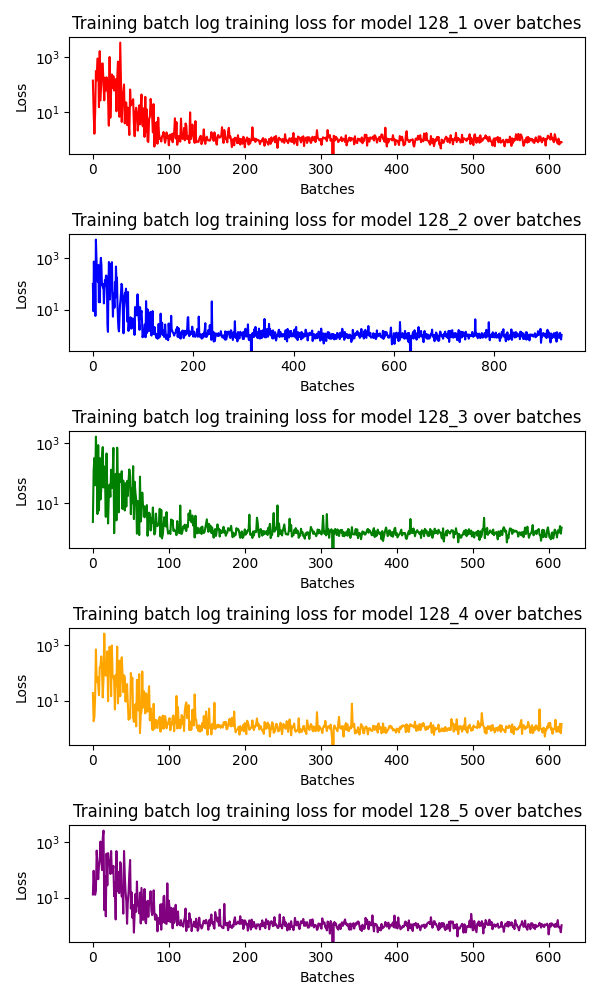
\includegraphics[width=0.95\linewidth]{Images/Results/Training_loss_128.png}
        \caption{1a}
        \label{fig:t-loss-128}
    \end{subfigure}%
    \begin{subfigure}{0.5\textwidth}
        \centering
        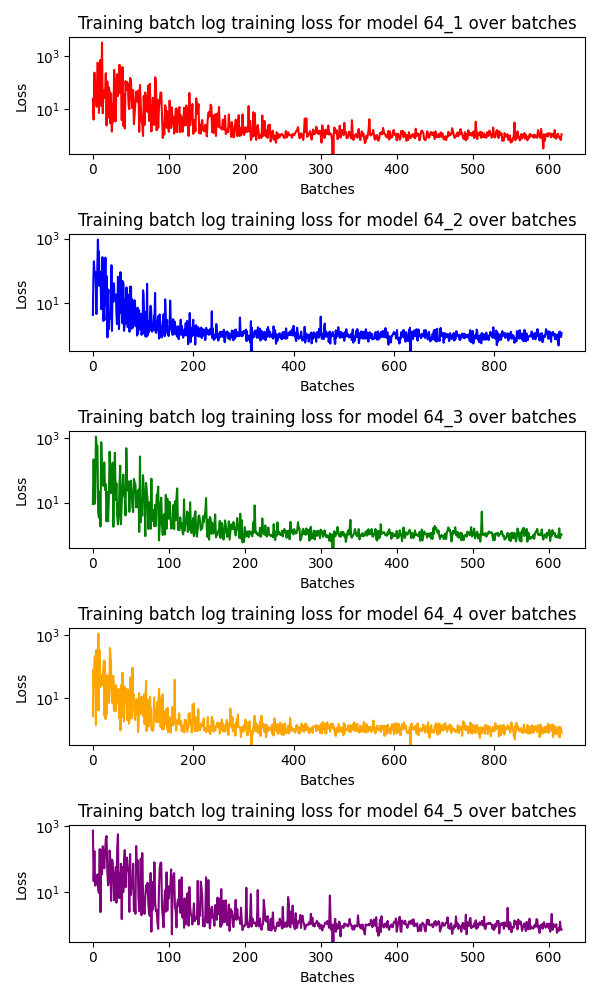
\includegraphics[width=0.95\linewidth]{Images/Results/Training_loss_64.png}
        \caption{1b}
        \label{fig:t-loss-64}
    \end{subfigure}
    \label{fig:t-loss}
\end{figure}

\begin{figure}[H]
    \caption{Plots of training loss for individual models in the ensembles of 64-state- and 128-state- representations.}
    \begin{subfigure}{0.5\textwidth}
        \centering
        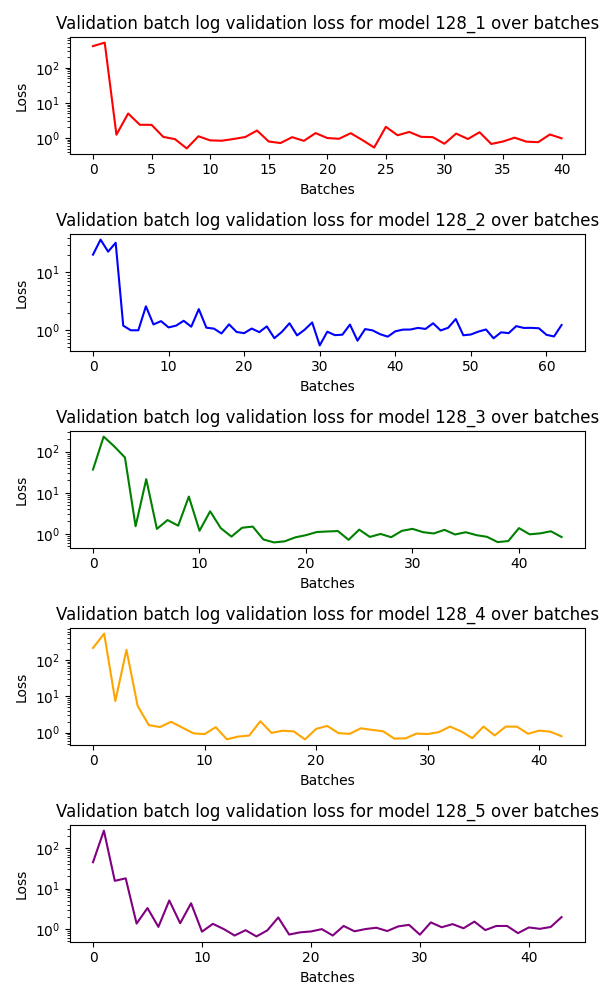
\includegraphics[width=0.95\linewidth]{Images/Results/Validation_loss_128.png}
        \caption{1a}
        \label{fig:v-loss-128}
    \end{subfigure}%
    \begin{subfigure}{0.5\textwidth}
        \centering
        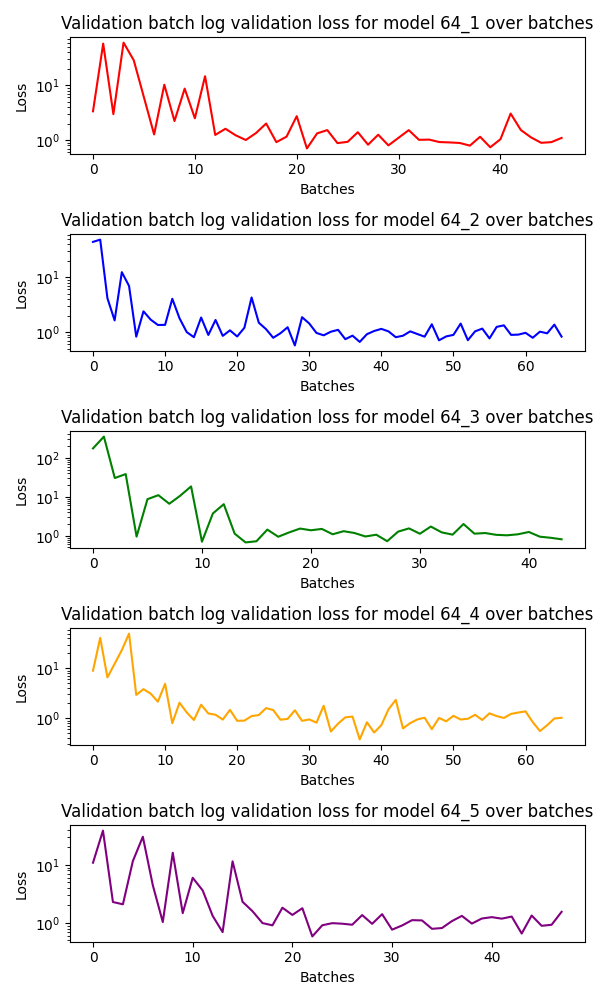
\includegraphics[width=0.95\linewidth]{Images/Results/Validation_loss_64.png}
        \caption{1b}
        \label{fig:v-loss-64}
    \end{subfigure}
    \label{fig:v-loss}
\end{figure}

\newpage



\section{Discussion}\label{sec:discussion}

%#TODO Fejlkilde: hyperparameter seach for kort, for lille datasæt, for få trials
%#TODO Nævn at høj for tidlig learning_rate ville få loss til at eksplodere, kombineret med for høj r_cut

%#TODO kom med en opsummering af kritik punkterne i et sidste afsnit.

\section{Conclusion}\label{sec:conclusion}
%#TODO opsummer forskningspørgsmålet, hvad scopet var og hvad vi satte ud for at gøre

%#TODO Konkluder på underpunkter

%#TODO Konkluder på overordnet forskningsspørgsmålet

%#TODO Future works sektion
\bibliographystyle{IEEEtran}
\bibliography{references_manually}
\newpage
\section{Appendix}\label{sec:appendix}

\subsection{Appendix A}\label{subsec:appendixA}

%#TODO write justification and explanation of hyperparameter selection

\subsection{Appendix B}\label{subsec:appendixB}

%#TODO write justification and explanation of hyperparameter selection


\subsection{Appendix C}\label{subsec:appendixC}

Two lists of main packages, and their versions vital to local development and cloud execution.
First the local development packages\ref{lis:localdev}:

\begin{itemize}\label{lis:localdev}
    \item Python 3.10.9
    \item Pytorch 2.0.1+cu118
    \item numpy 1.23.5
    \item pandas 1.5.2
    \item matplotlib 3.7.0
    \item tqdm 4.65.0
    \item python-dotenv 1.0.0
\end{itemize}

And for cloud execution\ref{lis:clouddev}:

\begin{itemize}\label{lis:clouddev}
    \item Python 3.9.14
    \item Pytorch 2.1.0+cu118
    \item numpy 1.23.5
    \item pandas 1.5.2
    \item scipy 1.9.1bstat
    \item tqdm 4.66.1
\end{itemize}



%\input{exempel_kode}



\end{document}
